\documentclass[bachelor, och, diploma]{SCWorks}
% параметр - тип обучения - одно из значений:
%    spec     - специальность
%    bachelor - бакалавриат (по умолчанию)
%    master   - магистратура
% параметр - форма обучения - одно из значений:
%    och   - очное (по умолчанию)
%    zaoch - заочное
% параметр - тип работы - одно из значений:
%    referat    - реферат
%    coursework - курсовая работа (по умолчанию)
%    diploma    - дипломная работа
%    pract      - отчет по практике
%    nir      - отчет о научно-исследовательской работе
%    autoref    - автореферат выпускной работы
%    assignment - задание на выпускную квалификационную работу
%    review     - отзыв руководителя
%    critique   - рецензия на выпускную работу
% параметр - включение шрифта
%    times    - включение шрифта Times New Roman (если установлен)
%               по умолчанию выключен
\usepackage[T2A]{fontenc}
\usepackage[cp1251]{inputenc}
\usepackage{graphicx}
\usepackage{tempora}
\usepackage{cmap}

\usepackage[sort,compress]{cite}
\usepackage{amsmath}
\usepackage{amssymb}
\usepackage{amsthm}
\usepackage{fancyvrb}
\usepackage{longtable}
\usepackage{minted}
\usepackage{array}
\usepackage[english,russian]{babel}


\usepackage[colorlinks=true]{hyperref}
\usepackage{pgfplots}
\pgfplotsset{compat=newest}% <-- moves axis labels near ticklabels (respects tick label widths)
\usepackage{listings}
\usepackage{color}
\usepackage{subfigure}

\definecolor{dkgreen}{rgb}{0,0.6,0}
\definecolor{gray}{rgb}{0.5,0.5,0.5}
\definecolor{mauve}{rgb}{0.58,0,0.82}

\setcounter{tocdepth}{4} 
\setcounter{secnumdepth}{4}


\newcommand{\eqdef}{\stackrel {\rm def}{=}}
\newcommand{\No}{\textnumero}
\newtheorem{lem}{Лемма}
\setminted{style=bw,
	linenos=true,
	breaklines=true,
	numbersep=5pt,
	tabsize=2,
	fontsize=\small,
	bgcolor=white}
\setmintedinline{style=bw,
	bgcolor=white,
	fontsize=\normalsize
	}	
\pgfplotsset{every axis legend/.append style={at={(0.6,1)},anchor=south west}}
%\pgfplotsset{every axis title/.style={at={(0.5,1)},above,yshift=6pt}}
\begin{document}

% Кафедра (в родительном падеже)
\chair{математической кибернетики и компьютерных наук}

% Тема работы
\title{Исследование индекса дружбы узлов растущих сетей построенных по моделям с предпочтительным присоединением}

% Курс
\course{4}

% Группа
\group{411}

% Факультет (в родительном падеже) (по умолчанию "факультета КНиИТ")
%\department{факультета КНиИТ}

% Специальность/направление код - наименование
\napravlenie{02.03.02 "--- Фундаментальная информатика и информационные технологии}
%\napravlenie{02.03.01 "--- Математическое обеспечение и администрирование информационных систем}
%\napravlenie{09.03.01 "--- Информатика и вычислительная техника}
%\napravlenie{09.03.04 "--- Программная инженерия}
%\napravlenie{10.05.01 "--- Компьютерная безопасность}

% Для студентки. Для работы студента следующая команда не нужна.
%\studenttitle{Студентки}

% Фамилия, имя, отчество в родительном падеже
\author{Козырева Юрия Дмитриевича}

% Заведующий кафедрой
\chtitle{к.\,ф.-м.\,н., доцент} % степень, звание
\chname{С.\,В.\,Миронов}

%Научный руководитель (для реферата преподаватель проверяющий работу)
\satitle{зав. каф., к.\,ф.-м.\,н., доцент} %должность, степень, звание
\saname{С.\,В.\,Миронов}

% Руководитель практики от организации (только для практики,
% для остальных типов работ не используется)
%\patitle{доцент, к.\,ф.-м.\,н.} 
%\paname{С.\,В.\,Миронов}

% Семестр (только для практики, для остальных
% типов работ не используется)
%\term{1}

% Наименование практики (только для практики, для остальных
% типов работ не используется)
%\practtype{учебная}

% Продолжительность практики (количество недель) (только для практики,
% для остальных типов работ не используется)
%\duration{16}

% Даты начала и окончания практики (только для практики, для остальных
% типов работ не используется)
%\practStart{01.09.2019}
%\practFinish{31.12.2019}

% Год выполнения отчета
\date{2023}

\maketitle

% Включение нумерации рисунков, формул и таблиц по разделам
% (по умолчанию - нумерация сквозная)
% (допускается оба вида нумерации)
%\secNumbering


\tableofcontents

% Раздел "Обозначения и сокращения". Может отсутствовать в работе
%\abbreviations

% Раздел "Определения". Может отсутствовать в работе
%\definitions

% Раздел "Определения, обозначения и сокращения". Может отсутствовать в работе.
% Если присутствует, то заменяет собой разделы "Обозначения и сокращения" и "Определения"
%\defabbr

% Раздел "Введение"
\intro
В повседневной жизни для решения многих задач часто используются случайные графы. Случайные графы нашли практическое применение во всех областях, где нужно смоделировать сложные сети. Имеется большое число моделей случайных графов, отражающих разнообразные типы сложных сетей в различных областях. Случайные графы применяются при моделировании и анализе биологических и социальных систем, сетей, а также при решении многих задач класса NP.

Случайные графы впервые определены венгерскими математиками \linebreak П.\,Эрдёшем и А.\,Реньи в книге 1959 года <<On Random Graphs>>\cite{RG}  и независимо американским математиком, Э.\,Гильбертом, в его статье <<Random graphs>>\cite{RG1}.

Случайный граф "--- общий термин для обозначения вероятностного распределения графов \cite{wico}. Их можно описать просто распределением вероятности или случайным процессом, создающим эти графы. 

Теория случайных графов находится на стыке комбинаторики, теории графов и теории вероятностей. В основе ее лежит глубокая идея о том, что мощные инструменты современной теории вероятностей должны поспособствовать более верному осознанию природы графа, призваны помочь решению многих комбинаторных и теоретико"=графовых задач \cite{habr}.

С математической точки зрения случайные графы необходимы для ответа на вопрос о свойствах типичных графов. Для этого используются модели Эрдёша"--~Реньи, Барабаши"--~Альберт, модель триадного замыкания, модель Бьянкони-Барабаши и другие. Все модели основываются на различных свойствах социальных сетей.

В дипломной работе рассматриваются одни из активно используемых и хорошо изученных моделей: модель Барабаши-Альберта и модель триадного замыкания.  

Для изучения и анализа моделей случайных графов, анализе социальных явлений и сетей, сообществ и их взаимодействий широко применяется индекс дружбы. Индекс дружбы "--- один из показателей, используемых в социологии, определяется как отношение средней степени соседей к степени самого объекта. 

Целью настоящей работы является анализ индекса дружбы сетей, построенных по модели Барабаши"--~Альберт. Для достижения этой цели необходимо решить следующие задачи.
\begin{itemize}
\item рассмотреть алгоритмы Барабаши"--~Альберт и триадного замыкания для построения случайного графа;
\item реализовать классический алгоритм Барабаши"--~Альберт, и его модификацию, в которой начальная степень каждого нового узла определяется как случайная величина, заданная пуассоновским распределением;
\item реализовать алгоритм триадного замыкания;
\item рассмотреть возможность параллельной реализации процесса получения случайного графа и  вычисления индекса дружбы;
\item организовать серии экспериментов, в которых строятся случайные графы по реализованным моделям; 
\item провести анализ распределения индекса дружбы построенных графов.
\end{itemize}




\section{Теоретические сведения}

Существует множество различных моделей построения случайных графов. Рассмотрим некоторые из них.
\subsection{Модель Эрдеша"--~Ренье}
Модель Эрдеша"--~Ренье является одной из первых моделей случайного графа. Граф построенный по этой модели представляет собой совокупность множества вершин $ V=\{1,...,n\} $ и множества рёбер $ E $, состоящего из рёбер полного графа $ K_{n} $ построенного на множестве $ V $, выбранных по схеме Бернулли. Таким образом образуется случайный граф $ G=(V, E) $. Формально выражаясь, мы имеем вероятностное пространство
\[
G(n, p)=(\Omega_n, F_n, P_{n, p}),
\] 
в котором: $n$ "---количество вершин, $p$ "---вероятность появления нового ребра, $F_n$ "---сигма-множество,$ \Omega_n$ "---множество возможных рёбер ($ |\Omega_n\ |=2^n$),  $P_{n,p}\ (G)=p^{|E|} (1-p)^{\binom{n}{2}-|E|}\ $ "---вероятностная мера.
Таким образом, в модели Эрдеша"--~Реньи каждое ребро независимо от других ребер входит в случайный граф с вероятностью $p$. Модель Эрдеша"--~Реньи на данный момент является самой изученной моделью случайных графов\cite{rey2}.
\subsection{Модель Барабаши"--~Альберт}
Модель Барабаши"--~Альберт является одной из первых моделей веб"=гра\-фов. Веб-граф представляет собой ориентированный мульти-граф, вершинами в котором являются какие-либо конкретные структурные единицы в Интернете: речь может идти о страницах, сайтах, хостах, владельцах и пр. Для определенности будем считать, что вершинами веб-графа служат именно сайты. А рёбрами соединяются вершины, между которыми имеются ссылки.

В своей модели А.-Л.\,Барабаши и Р.\,Альберт предложили стратегию предпочтительного присоединения\cite{BA}. Её основная идея  заключается в том, что вероятность присоединения конкретной вершины ребром к новой вершине пропорциональна степени данной вершины. Здесь и далее степенью вершины $v_i \in V$ графа $G = (V, E)$ называется количество вершин, напрямую связанных с данной, т.е. \[deg(v_i) = |\{v \in V: (v, v_i) \in E \}|.\] 

Алгоритм формирования сети по модели Барабаши"--~Альберт заключается в следующем.
\begin{enumerate}
\item Первоначально берется полный граф из $ m $ вершин, где $ m $ "--- параметр модели. 
\item На каждой итерации роста сети добавляется одна новая вершина, которая соединяется $ m $ ребрами с уже имеющимися в соответствии с принципом предпочтительного присоединения.
\end{enumerate}
 
\subsection{Модель Боллобаша"--~Риордана}
Одной из наиболее удачных и часто используемых моделей предпочтительного присоединения является модель Боллобаша"--~Риордана. Существуют две основных и, по сути, совпадающих модификации этой модели. В одной дается динамическое, а в другой статическое описание случайности\cite{rey1}.

В динамической модификации при добавлении $ n $-ной вершины проводятся $ n $ новых рёбер, при этом рёбра могут быть кратными, а также петлями. При создании графа с единственной вершиной проводится петля в этой точке\cite{rey2}. Таким образом вероятность появления ребра $ (n,\ i),\ \ i\in[0,\ n-1] $ равна $ \frac{deg_i}{2n-1} $, где $ deg_i $ "---степень вершины $i$. 

Статическая модель (LCD-модель) основывается на объекте называемом линейной хордовой диаграммой (LCD). Для построения данного объекта требуется зафиксировать на оси абсцисс $ 2n $ точек $ {1,…,2n} $, разбить их на пары и соединить элементы каждой пары дугой, лежащей в верхней полуплоскости. Количество различных диаграмм равно
\[
l_n=\frac{(2n)!}{2^nn!}. 
\]
По каждой диаграмме строится граф с $ n $ вершинами и $ n $ ребрами по следующему алгоритму: 
\begin{itemize}
\item Идти слева направо по оси абсцисс пока не встретится правый конец какой-либо дуги, пусть позиция этой точки равна $ i_k $
\item Последовательность $ i_{k-1}+1$, $i_k $ объявляется списком смежности для $k$-той вершины, $ i_0=0 $
\item Если $ k<n $, $ k $ увеличивается на 1, переход на шаг (1).
\end{itemize}
	
При построении модели LCD случайно выбирается одна из возможных LCD и вероятность каждой диаграммы равной $ \frac{1}{l_n} $, где $ l_n $ – общее число диаграмм. Графы построенные по такой модели имеют те же свойства, что и графы построенные по динамической модификации схемы Боллобаша"--~Риордана.
\subsection{Модель Чунг-Лу}
Пусть нам задано некоторое конечное множество вершин $ V ={v_1 ,… , v_n}  $ и степень каждой вершины $ d_i$, $i=\overline{1,n} $. Генерация графа $ G = (V, E) $ происходит следующим образом:
\begin{itemize}
\item формируем множество $ L $, состоящее из $ i \cdot d $ копий $ i \cdot v $ для каждого $ i $ от $ 1 $ до $ n $;
\item задаем случайные паросочетания на множестве $ L $;
\item для вершин $ u $ и $ v $ из $ Vs $ количество ребер в графе $ G $ , соединяющее их, равно числу паросочетаний между копиями $ u $ и $ v $ в $ L $\cite{article}.
\end{itemize}
Сгенерированный таким образом граф соответствует степенной модели $ P(a,b) $, описывающей графы, для которых:
\[
|\{v|\deg_v=\ x\}|=\frac{e^\alpha}{e^\beta}. 
\]
\subsection{Модель триадного замыкания}
Помимо стратегии предпочтительного присоединения, модель триадного замыкания использует стратегию формирования триад. Триадное замыкание "---свойство социальных систем заключающееся в том, что если между вершинами (A, B) и (A, C), в некоторой социальной сети существует взаимосвязь, то велика вероятность формирования триады из этих трёх вершин, т.е., велика вероятность связи (B, C) \cite{ts}.  В модели триадного замыкания рост сети происходит следующим образом.
\begin{enumerate}
\item Первоначально берется полный граф из $ m $ вершин, где $ m $ "--- параметр модели. 
\item На каждой итерации роста сети добавляется одна новая вершина, которая соединяется $ m $ ребрами с уже имеющимися  по следующим правилам:
\begin{itemize}
\item в соответствии с принципом предпочтительного присоединения выбирается вершина, к которой проводится первое ребро;
\item с вероятностью $ p $, где $ p $ "--- параметр модели, выбирается стратегия формирования триады с произвольным соседом вершины, присоединенной первым ребром, или, с вероятностью $ (1-p) $, стратегия предпочтительного присоединения к произвольной вершине графа.
\end{itemize}
\end{enumerate}

\subsection{Индекс дружбы}

С момента появления социальных сетей  — Facebook, Vkontakte, LiveJournal, Instagram, LinkedIn, MySpace и т. д. прошло не так много времени, но они уже плотно вошли в повседневную жизнь многих людей.

Опросы показывают, что 76\% пользователей Интернета в России (по данным агентства PRT на январь 2014) и примерно 73\% жителей Соединенных Штатов являются активными пользователями социальных сетей, и эта цифра растет\cite{psych}.

В современном обществе социальные сети становятся огромной базой информации, которую ученые и работодатели все чаще привлекают для решения конкретных задач, будь то научное исследование или оценка кандидата на определенную должность.

Научный интерес к изучению пользователей социальных сетей стремительно растет. На данный момент накоплено большое количество эмпирического материала в отношении характеристик пользователей социальных сетей, который требует систематизации и осмысления.

В социальных сетях часто можно встретить явление именуемое парадоксом дружбы: в среднем друзья любого человека имеют больше друзей, чем он сам. Оно было обнаружено в 1991 году социологом из государственного университета Нью-Йорка Скоттом Фельдом\cite{aw}.

Для изучения парадокса дружбы следует ввести несколько обозначений. В момент времени $t$ для вершины $v_i$ в графе $G(t) = (V(t), E(t))$ сумма степеней всех соседей $v_i$ равна:
\[
s_i(t) = \sum_{j: (v_i, v_j ) \in E(t)} deg_j(t),
\]
средняя степень соседей0 вершины $ v_i $:
\[
\alpha_i(t) = \dfrac{s_i(t)}{deg_i(t)}, 
\]
а индекс дружбы $\beta_i(t)$ определяется как отношение средней степени соседей $v_i$ к степени самой $v_i$: 
\[
\beta_i(t) = \dfrac{\alpha_i(t)}{deg_i(t)} = \dfrac{s_i(t)}{deg_i^2 (t)} = \dfrac{\sum_{j: (v_i, v_j ) \in E(t)} deg_j(t)}{deg_i^2 (t)}.
\]

Таким образом, если средняя степень соседей больше степени $v_i$ и парадокс дружбы выполняется, то $\beta_i(t) > 1$ \cite{fi}.

Для примера, социальные сети Facebook и Github подтверждают парадокс дружбы, что показано на Рис.\,\ref{fig:img3} \cite{mir}.
Здесь на оси $ Oy $  отложено количество узлов сети, для которых индекс дружбы $ \beta_i $ попадает в диапазон, отложенный на оси $ Ox $. Как видим, значительное большинство вершин графов имеют значение индекса дружбы большее единицы.   
\begin{figure}[!ht]
    \centering
    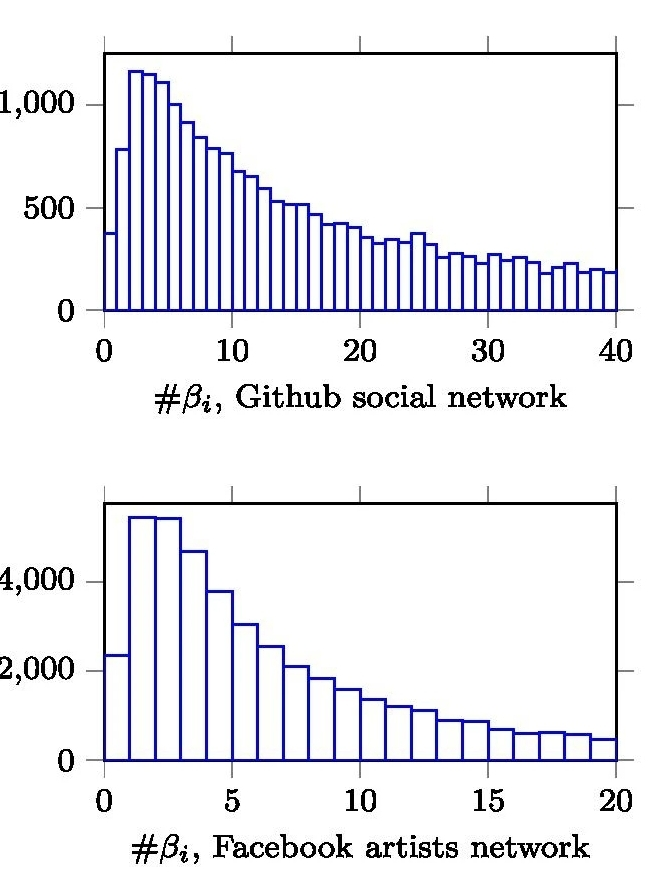
\includegraphics[scale=0.4]{examples1.jpg}
    \caption{Распределения индекса дружбы в\\ сети телефонных звонков и сети доставки Amazon}\label{fig:img3}
\end{figure}

\section{Реализация моделей}
В ходе выполнения дипломной работы были реализованы: стандартная модель Барабаши"--~Альберт, модель Барабаши"--~Альберт с пуассоновским распределением начальных степеней и модель триадного замыкания. Все расчёты производились на компьютере с процессором Intel core i5-8265U и 16 ГБ оперативной памяти. Модель реализована на Python 3.9.1. При реализации использовались библиотеки json, multiprocessing, random и numpy.random.

Все три реализованные модели представляют собой модели растущего случайного графа с использованием механизма предпочтительного присоединения. В реализованных модификациях на каждом шаге добавляется одна вершина и некоторое количество $m$ рёбер, при этом параметр $m$ и процесс выбора соседей новой вершины зависят от используемой модели. В модели триадного замыкания используется дополнительный параметр $ p $. 

В экспериментах перебираются различные модели и различные значения параметров. В каждом эксперименте строится граф из 100000 вершин. Так как получаемые графы случайны, то в ходе эксперимента граф строится десять раз, после чего строится усреднённая гистограмма по диапазонам значений индекса дружбы и график динамики изменений среднего индекса дружбы графа.

В реализации моделей граф описывается парой массивов \mintinline{py}{degrees} и \mintinline{py}{neibours}, хранящие соответственно степень и список номеров соседних вершин для каждой вершины графа. Каждая модель реализована в форме функции\\ \mintinline{py}{model_name(n, args, funcs, dts)},\\ где параметр \mintinline{py}{n} задаёт размер конечного графа, массив \mintinline{py}{args} содержит аргументы модели, \mintinline{py}{funcs} является массивом метрик, которые нужно применить к графу, а \mintinline{py}{dts} "---периодичность применения метрик. 

Метрики также представлены функциями вида\\ \mintinline{py}{metric_name(degrees, neibours)},\\ в которых \mintinline{py}{degrees} представляет собой массив степеней вершин графа, а \mintinline{py}{neibours} "---массив массивов соседних вершин. В ходе работы были использованы четыре метрики:
\begin{itemize}
\item \mintinline{py}{s(degrees, neibours)} "---возвращает массив сумм степеней соседей для вершин графа;
\item \mintinline{py}{alfa(degrees, neibours)} "---возвращает массив средних степеней соседей для вершин графа;
\item \mintinline{py}{beta(degrees, neibours)} "---возвращает массив индексов дружбы для  вершин графа;
\item \mintinline{py}{mean_beta(degrees, neibours)} "---возвращает средний индекс дружбы всего графа
\end{itemize}
\subsection{Реализация стандартной модели Барабаши"--~Альберт}
Реализация стандартной модели Барабаши "--~ Альберт состоит в следующем. 

Модель реализована в виде функции\\
\mintinline{py}{my_bag(n, args, funcs, dts)},\\
как описано выше.

В качестве параметра $m$ модели принимается нулевой элемент массива \mintinline{py}{args}. 

В ходе реализации используется массив \mintinline{py}{ans}, в котором будут хранится значения метрик построенного графа, он заполняется пустыми массивами по количеству метрик: \linebreak\mintinline{py}{ans = [[] for _ in range(len(dts))]}.

Создаётся полный граф из $ m + 1$ вершин. Для этого массив \mintinline{py}{degrees} заполняется \mintinline{py}{m + 1} значениями \mintinline{py}{m} и массив \mintinline{py}{neibours} формируется из \mintinline{py}{m + 1} списков, каждый из которых содержит номера всех существующих в данный момент вершин в графе, кроме текущей.
\begin{minted}{python}
		degrees = list(np.full(m + 1, m))
    neibours = [list(np.delete(np.arange(m + 1), i)) for i in np.arange(m + 1)]
\end{minted}
Далее создаются вспомогательные массивы \mintinline{py}{nodes}, содержащие список номеров всех вершин содержащихся в графа на данный момент, и \mintinline{py}{used} "--- массив, в котором отмечаются вершины графа, уже присоединенные к новому узлу. 
\begin{minted}{python}
		nodes = np.arange(m + 1)
    used = np.full(n, False)
\end{minted}

Затем в цикле по $n - (m + 1)$ индексам к графу присоединяются новые вершины. Для хранения соседей нового узла формируется список \mintinline{py}{conections}. С помощью функции \mintinline{py}{random.choices} выбираются $m$ уникальных вершин, которые записываются в \mintinline{py}{conections}. Уникальность вершин определяется по списку \mintinline{py}{used}, принцип предпочтительного присоединения соблюдается благодаря передаче степеней вершин в качестве массива весов в \mintinline{py}{random.choices}.
\begin{minted}{python}
while j < m:
    choosen = random.choices(nodes, weights = degrees, k = 1)[0]
    if not used[choosen]:
        j += 1
        conections.append(choosen)
        used[choosen] = True
\end{minted}

В следующем цикле по элементам массива \mintinline{py}{connections}  в массиве \mintinline{py}{used} все \mintinline{py}{True} заменяются на \mintinline{py}{False}. Кроме того, значения списка \mintinline{py}{neibours} дополняются образованными на данном шагу связями, соответственно изменяется массив \mintinline{py}{degrees}. 
\begin{minted}{python}
for j in conections:
    used[j] = False
    neibours[i + 1].append(j)
    neibours[j].append(i)
    degrees[j] += 1
degrees.append(m)
\end{minted}

Последним этапом добавления новой вершины в данном алгоритме является сбор метрик графа в текущем состоянии. Для каждой функции в списке \mintinline{py}{funcs} алгоритм определяет, нужно ли снимать данную метрику на данном шаге, основываясь на проверке делимости \mintinline{py}{i} на соответствующее значение \mintinline{py}{dts}. Если текущая метрика запрошена пользователем на данном шаге, то результат её обсчёта добавляется в соответствующую ячейку массива \mintinline{py}{ans}. 
\begin{minted}{python}
for j in range(len(dts)):
    if i % dts[j] == 0:
        ans[j].append(funcs[j](degrees, neibours))
\end{minted}

Результатом выполнения всей функции \mintinline{py}{my_bag} является \mintinline{py}{ans}.

\subsection{Реализация модели Барабаши"--~Альберт со случайным числом добавляемых рёбер на каждой итерации}
Реализация модели Барабаши"--~Альберт с пуассоновским распределением степеней новых вершин во многих аспектах повторяет стандартную модель Барабаши"--~Альберт. Первое отличие заключается в содержимом списка параметров \mintinline{py}{args}: вместо параметра $m$ данная модель принимает параметр $\lambda$ для распределения Пуассона. Этот параметр извлекается в переменную \mintinline{py}{m} и используется для генерации значения \mintinline{py}{m0} "--- количества вершин начального полного графа. 
\begin{minted}{python}
		m = args[0]
    ...
    m0 = np.random.poisson(m)
    degrees = list(np.full(m0 + 1, m0))
    neibours = [list(np.delete(np.arange(m0 + 1), i)) for i in np.arange(m0 + 1)]    
\end{minted}

Начальные степени каждой новой вершины также определяются в соответствии с распределением Пуассона. Так как степень новой вершины не может быть ни больше чем количество узлов графа, ни меньше единицы, то на число соседей новой вершины нужно наложить соответствующие ограничения.
\begin{minted}{python}
		mi = max(1, min(np.random.poisson(m), nodes.shape[0]))
\end{minted}
\subsection{Реализация модели триадного замыкания}
Модель триадного замыкания также реализована как модификация стандартной модели Барабаши"--~Альберт. В отличие от других реализованных моделей список аргументов содержит два параметра: фиксированная степень новых вершин $m$ и вероятность образования триады $p$, они извлекаются в переменные с соответствующими названиями.
\begin{minted}{python}
		m = args[0]
    p = args[1]
\end{minted}

Также вносятся определённые изменения в процесс добавления новых вершин: в данной вариации существуют два способа выбора кандидата \mintinline{py}{choosen} на роль нового соседа текущего узла. Выбор по принципу предпочтительного присоединения производится либо с вероятностью $1-p$ из множества всех вершин графа, либо из числа соседей вершины присоединённой первой. Первый узел присоединяется также в соответствии с первым вариантом.
\begin{minted}{python}
if j == 0 or np.random.rand() > p:
    choosen = random.choices(nodes, weights = degrees, k = 1)[0]
else:
    choosen = random.choices(neibours[conections[0]], k = 1)[0]
\end{minted}
\subsection{Паралелизация построения модели Барабаши"--~Альберт}
Для ускорения работы программы была реализована многопоточная версия алгоритма с помощью библиотек multiprocessing и  numpy: функция \mintinline{py}{run} создаёт потоки, распределяет задания и собирает результаты, а функция \linebreak \mintinline{py}{run_thread} проводит эксперементы в каждом потоке отдельно и возвращает их результат.

Функция \mintinline{py}{run} принимает семь аргументов: количество случайных графов, которые требуется построить, \mintinline{py}{N}; количество потоков \mintinline{python}{thread}, алгоритм построения случайного графа \mintinline{python}{model}; размер графов \mintinline{python}{n}; массив аргументов модели \mintinline{python}{args}; список метрик \mintinline{python}{funcs} и частоты их снятия \mintinline{python}{dts}. Сначала создаётся объект класса \mintinline{py}{multiprocessing.Manager}, который будет управлять в дальнейшем созданными потоками, ссылка на словарь с результатами вычислений - \mintinline{py}{manager.dict()} хранится в переменной \mintinline{py}{res}. Затем в цикле для каждого из \mintinline{py}{thread} ядер создаётся свой \mintinline{py}{multyprocessing.Process} который будет выполнять соответствующий поток. Все процессы добавляются в список выполняющихся потоков и запускаются, с помощью метода \mintinline{py}{p.start}. Далее мы дожидаемся выполнения всех потоков, собираем все результаты в список \mintinline{py}{ans} и возвращаем его как результат функции.

Первым шагом в \mintinline{py}{run_thread} инициализируется пустой список \mintinline{py}{ans}. Потом поочерёдно строится заданное колличество случайных графов, для каждого из них вычисляется заданная метрика и результат записывается в список  \mintinline{py}{ans}.
\begin{minted}{python}
def run_thread(N, i, res, model, n, args, funcs, dts):
    ans = []
    for j in range(N):
        ans.append(model(n, args, funcs, dts))
    res[i] = ans
def run(N, treads, model, n, args, funcs, dts):
    procs = []
    manager = multiprocessing.Manager()
    res = manager.dict()
    for i in range(treads):
        curn = min(N, math.ceil(N / (treads - i)))
        p = multiprocessing.Process(target=run_thread, args=(curn, i, res, model, n, args, funcs, dts))
        N -= curn
        procs.append(p)
        p.start()
    for proc in procs:
        proc.join()
    ans = []
    for i in res.values():
        ans += i
    return ans
\end{minted}
\subsection{Вывод и представление данных для анализа}
Данная реализация содержит фрагмент кода, отвечающий за отображение данных о построенном графе для дальнейшего анализа. Для этого используются библиотеки matplotlib, matplotlib.pyplot\cite{ptl} и numpy. 

В ходе проведения экспериментов для каждой модели каждые 100 итераций замерялся средний индекс дружбы вершин графа, а так же после построения графа вычислялся индекс дружбы для каждой из вершин с целью отображения распределения его значений. 

Сначала обрабатываются данные финального индекса дружбы, они представлены в виде трёхмерного массива: для каждого построенного графа, для каждого такта снятия метрик, для каждой вершины имеется значения индекса дружбы. Так как данные снимаются лишь однажды то измерение тактов можно убрать оставив от него лишь элементы на нулевых позициях. Затем для каждого графа  строится гистограмма, значения столбцов гистограммы усредняются по набору графов. По усреднённой гистограмме строится график и результат сохраняется. 
\begin{minted}{python}
ans = run(10, 6, my_triad, n, [m, p], [beta, mean_beta], [n - 1, 100])
beta_data = np.array([i[0] for i in ans])
beta_data = [np.histogram(i[0], bins=100) for i in beta_data]
beta_data = [[i[0], np.delete(i[1], 100)] for i in beta_data]
beta_data = np.array(beta_data)
beta_data = beta_data.transpose((1, 2, 0))
beta_data = np.apply_along_axis(arr = beta_data, axis = 2, func1d = np.mean)
plt.bar(beta_data[1], beta_data[0])
plt.savefig('\\source\\repos\CSW\\diploma_results\\triad_beta_' + str(m) + '.jpg')
plt.clf()
\end{minted}

Схожим образом преобразуется информация о динамике среднего индекса дружбы. Она хранится в массиве \mintinline{py}{ans} под индексом \mintinline{py}{1} и выносится в список \mintinline{python}{mean_beta_data}. Измерение графов и измерение тактов меняются местами. Затем данные усредняются по графам, по ним строится и сохраняется график.
\begin{minted}{python}
mean_beta_data = np.array([i[1] for i in ans])
mean_beta_data = np.apply_along_axis(arr=mean_beta_data, axis=2, func1d=lambda x: x[0])
mean_beta_data = mean_beta_data.transpose((1, 0))
mean_beta_data = np.apply_along_axis(arr=mean_beta_data, axis=1, func1d=mean)
plt.bar(mean_beta_data, np.arange(mean_beta_data.shape[0]))
plt.savefig('\\source\\repos\\CSW\\diploma_results\\triad_mean_beta_' + str(m) + '.jpg')
plt.clf()
\end{minted}

Эта последовательность повторяется для каждой модели графа, для каждой комбинации параметров.
\begin{minted}{python}
for m in [3, 5]:
    for p in [0.25, 0.5, 0.75]:
  				ans = run(10, 6, my_triad, n, [m, p], [beta, mean_beta], [n - 1, 100])
      ...
      plt.clf()
for m in [3, 5]:
   		ans = run(10, 6, my_bag, n, [m, p], [beta, mean_beta], [n - 1, 100])
      ...
      plt.clf()
for m in [4, 5, 6]:
   		ans = run(10, 6, my_bag_poisson, n, [m, p], [beta, mean_beta], [n - 1, 100])
      ...
      plt.clf()
\end{minted}

Кроме того, необходимо построить и сохранить в текстовый документ по одному экземпляру каждого графа для дальнейшего изучения. В качестве текстового формата хранения графа был выбран формат json, в силу его структурированности, читабельности для человека, простоты для чтения и записи. В json-файле граф представляется как список словарей, каждый элемент списка представляет вершину графа. Вершина представлена тремя записями словаря: 
\begin{itemize}
\item \mintinline{js}{index} "--- индекс вершины в графе,
\item \mintinline{js}{degree} "--- степень вершины, 
\item \mintinline{js}{neibours} "--- список соседей узла. 
\end{itemize} 

Так как алгоритмы построения графа возвращают не граф целиком, а только значения заданных метрик, то данные графа необходимо извлекать с помощью псевдометрик \mintinline{py}{d}, \mintinline{py}{neibours} и \mintinline{py}{index}, они возвращают массив степеней, матрицу соседей и список индексов графа, соответственно. Эти значения сохраняются в файл.
\begin{minted}{python}
def d (degrees, neibours):
    return degrees
def neibours (degrees, neibours):
    return neibours
def index (degrees, neibours):
    return np.arange(len(neibours))
...
						ans = run(1, 6, my_triad, n, [m, p], [index, d, neibours], [n - 1, n - 1, n - 1])
            ans = ans[0]
            ans = [i[0] for i in ans]
            prejson = [{'index':int(ans[0][i]), 'degree':int(ans[1][i]), 'neibours':[int(j) for j in ans[2][i]]} for i in range(len(ans[0]))]
            with open('\\source\\repos\\CSW\\diploma_results\\triad_graph_' + str(m) + '_' + str(p) + '.json', 'w') as f:
                json.dump(prejson, f)
                f.close()
    
\end{minted}

В результате для каждого графа получается json-файл следующего вида:
\begin{minted}{js}
[{"index": 0, "degree": 799, "neibours": [1, 2, ... , 99033]}, 
{"index": 1, "degree": 1032, "neibours": [0, 2, 3, ... , 99996]}, 
{"index": 2, "degree": 418, "neibours": [0, 1, 3, ... , 99864]}, 
{"index": 3, "degree": 624, "neibours": [0, 1, 2, ... , 99859]}, 
{"index": 4, "degree": 437, "neibours": [0, 1, 2, ... , 99922]}, 
{"index": 5, "degree": 174, "neibours": [4, 0, 1, 13, ... , 99982]},
...
{"index": 100000, "degree": 3, "neibours": [22224, 691, 5888]}]
\end{minted}
Полный код программы приведен в приложении~\ref{app:program}.
\section{Анализ графов реальных сетей}
В ходе выполнения дипломной работы были написаны несколько скриптов для считывания из текстового файла и анализа графов реальных сетей:
\begin{itemize}
\item скрипт для эффективного считывания больших сетей (до нескольких миллионов вершин и десятки миллионов рёбер) и вычисления распределения индекса дружбы в них;
\item программа для чтения графов с информацией о времени появления ребра и отслеживания динамики изменения среднего индекса дружбы;
\item скрипт читающий два файла: файл с рёбрами и файл содержащий данные о времени добавления вершины, и также отображающий динамику усреднённого индекса дружбы графа.
\end{itemize}
\subsection{Скрипт для отображения распределения индекса дружбы}
Так как скрипт для отображения распределения индекса дружбы должен обрабатывать большие графы при ограниченном количестве памяти, то становится невозможным сохранить всю информацию о графе. Однако для подсчёта индекса дружбы необходимы данные о соседях каждой вершины, потому что в процессе считывания граф постоянно меняется и высчитать индекс дружбы при добавлении вершины или обновлять его динамически становится невозможно. Данная проблема была решена при помощи двукратного прохода по считываемому файлу: один для подсчёта конечных степеней всех вершин, и второй для для передачи этих данных соседям, так данный алгоритм не подразумевает хранения данных о рёбрах графа.

Сначала скрипт открывает на чтение нужный файл, создаются список под значения индекса дружбы "--- \mintinline{py}{res} и словарь \mintinline{py}{degrees} для хранения степеней вершин.
\begin{minted}{python}
file = open('\\source\\repos\\CSW\\real_graphs\\' + name + '.txt', 'r')
res = []
degrees = {}
\end{minted}
Затем запускается цикл считывания в котором строка из файла записывается в переменную \mintinline{py}{line}, если строка оказывается равной \mintinline{py}{null}, то цикл прерывается. Разбивая строку \mintinline{py}{line} по символу пробела формируется ребро \mintinline{py}{edge}. Для каждого из двух концов ребра к количеству соседей добавляется $1$, если для вершины ещё не существует записи в \mintinline{py}{degrees} то она создаётся и инициализируется $0$.
\begin{minted}{python}
while True:
    line = file.readline()
    if not line:
        break
    edge = [int(j) for j in line.split(" ")]
    if not edge[0] in degrees:
        degrees[edge[0]] = 0
    degrees[edge[0]] += 1
    if not edge[1] in degrees:
        degrees[edge[1]] = 0
    degrees[edge[1]] += 1
\end{minted}
Затем курсор переводится в начало файла. Создаётся словарь \mintinline{py}{sum} для сумм соседей каждой вершины. И запускается второй цикл считывания аналогичный первому, с единственным отличием в том, что он насчитывает суммы соседей, а не степени вершин.
\begin{minted}{python}
file.seek(0)
sums = {}
while True:
    line = file.readline()
    if not line:
        break
    edge = [int(j) for j in line.split(" ")]
    if not edge[0] in sums:
        sums[edge[0]] = 0
    sums[edge[0]] += degrees[edge[1]]
    if not edge[1] in sums:
        sums[edge[1]] = 0
    sums[edge[1]] += degrees[edge[0]]
\end{minted}
В завершении программы для каждой вершины определяется индекс дружбы, файл закрывается, после чего строится и сохраняется гистограмма распределения индекса дружбы в заданном графе. 
\begin{minted}{python}
for i in degrees.keys():
        res.append(sums[i] / degrees[i] / degrees[i])
file.close()
bincnt = 100000
ans = np.histogram(res, bincnt)
x = ans[1]
y = ans[0]
x = np.resize(x, x.size - 1)
plt.bar(x[0:int(bincnt / 100 * 2)], y[0:int(bincnt / 100 * 2)])
plt.savefig("\\source\\repos\\CSW\\diploma_results\\" + name + "_static.jpg")
plt.clf()
\end{minted}
Полный код скрипта представлен в приложении~\ref{app:rgs}.
\subsection{Скрипт для отображения динамики индекса дружбы}
Скрипт для отображения динамики индекса дружбы должен быть способен многократно высчитывать индекс дружбы на считываемом графе, поэтому он сохраняет не только списки соседей вершин, но также и суммы степеней соседей. 

Первые шаги напоминают предыдущий алгоритм: файл открывается на чтение и запускается цикл считывания. Однако данные записываются в список \mintinline{py}{edge_list} практически без обработки "--- строка просто разбивается по символу \mintinline{py}{\t}.
\begin{minted}{python}
file = open('\\source\\repos\\CSW\\real_graphs\\' + name, 'r')
    edge_list = []
    while True:
        line = file.readline()
        edge_list.append(line.split("\t"))
        if not line:
            break
    edge_list.pop()
\end{minted}
Затем элементы \mintinline{py}{edge_list} преобразуются в тройки чисел содержащие номер первой вершины ребра, номер второй вершины и unix-время добавления грани. Все данные из файла считаны и он закрывается.
\begin{minted}{python}
edge_list = [[i[0], 
              i[1], 
              datetime.datetime.strptime(i[3], '%Y-%m-%d %H:%M:%S').timestamp()] 
             for i in edge_list]
file.close()
\end{minted}
Полученный массив сортируется с помощью метода \mintinline{py}{list.sort()} в порядке возрастания временной метки. Инициализируются следующие переменные:
\begin{itemize}
\item шаг времени замера \mintinline{py}{step}, 
\item точка начала отсчёта времени \mintinline{py}{base}, 
\item список для хранения результатов \mintinline{py}{res},
\item словари которые будут содержать обрабатываемый граф:
\subitem \mintinline{py}{degrees} "--- словарь степеней графа;
\subitem \mintinline{py}{neibours_degrees} "--- содержит суммы степеней соседей;
\subitem \mintinline{py}{neibours} "--- множества самих соседей вершин.
\end{itemize}
\begin{minted}{py}
edge_list.sort(key = lambda i: i[2])
step = 1000
base = edge_list[0][2]
res = []
degrees = {}
neibours_degrees = {}
neibours = {}
\end{minted}
Следующим шагом в цикле по отсортированному массиву происходит проверка каждой вершины на наличие в уже описанной части графа, если если вершины ещё нет то для неё инициализируются записи во всех трёх словарях.
\begin{minted}{python}
for i in edge_list:
    cnt += 1
    if not i[0] in degrees:
        degrees[i[0]] = 0
        neibours[i[0]] = set()
        neibours_degrees[i[0]] = 0
    if not i[1] in degrees:
        degrees[i[1]] = 0
        neibours[i[1]] = set()
        neibours_degrees[i[1]] = 0
\end{minted}
Если вершина является петлёй то степень одного из концов увеличивается на $1$, к сумме степеней соседей данной вершины добавляется степень самой вершины, а суммы степеней соседей всех смежных вершин увеличиваются на $1$, наконец, происходит попытка добавить новую вершину в множество соседей (очевидно, попытка не удастся, если узел уже содержится в множестве).
\begin{minted}{python}
if i[0] == i[1]:
    degrees[i[0]] += 1
    neibours_degrees[i[0]] += degrees[i[0]]
    for j in neibours[i[0]]:
        neibours_degrees[j] += 1
    neibours[i[0]].add(i[0])
\end{minted}
В обратном случае к выше указанные шаги проводятся дважды (для каждого конца грани).
\begin{minted}{python}
else:
  degrees[i[0]] += 1
  degrees[i[1]] += 1
  if not i[1] in neibours[i[0]] and not i[0] in neibours[i[1]]:
      neibours_degrees[i[0]] += degrees[i[1]]
      neibours_degrees[i[1]] += degrees[i[0]]
  for j in neibours[i[0]]:
      neibours_degrees[j] += 1
  for j in neibours[i[1]]:
      neibours_degrees[j] += 1
  neibours[i[0]].add(i[1])
  neibours[i[1]].add(i[0])
\end{minted}
Когда с момента \mintinline{py}{base} проходит более \mintinline{py}{step} секунд, \mintinline{py}{base} обновляется до наименьшего значения превосходящего текущий момент времени. В список \mintinline{py}{ans} записываются значения индекса дружбы вершин графа. Эти значения усредняются с помощью \mintinline{py}{numpy.mean()} и среднее добавляется в \mintinline{py}{res}.
\begin{minted}{python}
if (i[2] - base) >= step:
    base = step * math.ceil(i[2] / step)
    ans = []
    for j in degrees.keys():
        ans.append(neibours_degrees[j] / degrees[j] / degrees[j])
    res.append(np.mean(ans))
\end{minted}
По значениям \mintinline{py}{res} строится и сохраняется график.
\begin{minted}{python}
plt.plot(res)
plt.savefig("\\source\\repos\\CSW\\diploma_results\\" + name + "_iterational_dynamics.jpg")
plt.clf()
\end{minted}
Так как скрипт не применялся к слишком объёмным графам, то в ходе его выполнения остаётся достаточное количество ресурсов для одновременной обработки нескольких сетей в многопоточном режиме.
\begin{minted}{python}
def run_thread(namegroup, i, res):
    ans = []
    for j in namegroup:
        ans.append(dynamics(j))
    res[i] = ans
def run(names):
    procs = []
    manager = multiprocessing.Manager()
    res = manager.dict()
    for (i, namegroup) in enumerate(names):
        p = multiprocessing.Process(target=run_thread, args=(namegroup, i, res))
        procs.append(p)
        p.start()
    for proc in procs:
        proc.join()
    ans = []
    for i in res.values():
        ans += i
    return ans
run([['askubuntu', 'askubuntu-a2q'], ['askubuntu-c2a', 'askubuntu-c2q'], ['mathoverflow', 'mathoverflow-a2q'], 
     ['mathoverflow-c2a', 'mathoverflow-c2q'], ['superuser', 'superuser-a2q'], ['superuser-c2a', 'superuser-c2q']])
\end{minted}
Полный код скрипта представлен в приложении~\ref{app:rg}.
\subsection{Скрипт для отображения динамики индекса дружбы в графах представленных в нескольких файлах}
Данная программа является модификацией предыдущей. Основное отличие заключается в том, что в данном случае время добавления вершин считывается из отдельного файла в словарь \mintinline{py}{times}.
\begin{minted}{python}
time_file = open('\\source\\repos\\CSW\\real_graphs\\' + name + '-dates.txt', 'r')
times = {}
while True:
    line = time_file.readline()
    if not line:
        break
    line = line.split("\t")
    line = [int(line[0]), int(line[1].replace('-', ''))]
    times[line[0]] = line[1]
\end{minted}
Кроме того, сортировка массива степеней \mintinline{py}{edge_list} проводится с помощью лямбда-функции, сопоставляющей вершину начала ребра с временем её добавления.
\begin{minted}{python}
edge_list.sort(key = lambda i: times[i[0]] if i[0] in times else 100000000)
\end{minted}
Полный код скрипта представлен в приложении~\ref{app:rgp}.
\section{Анализ}
Для того чтобы проверить, что реализованные модели могут выступать в качестве моделей социальных процессов в окружающем мире, нужно показать, что сгенерированные графы обладают некоторыми свойствами реальных сетей. В качестве характеристики для анализа был выбран индекс дружбы 
\[
\beta_i(t) = \dfrac{\alpha_i(t)}{deg_i(t)} = \dfrac{s_i(t)}{deg_i^2 (t)} = \dfrac{\sum_{j: (v_i, v_j ) \in E(t)} deg_j(t)}{deg_i^2 (t)}.
\]
В работе рассматривались распределение индекса дружбы и динамика его среднего значения.
\subsection{Анализ распределения и динамики индекса дружбы в построенных графах}
На графике, представленном на Рис.\,\ref{fig:bas3}, изображено распределение индекса дружбы в графе построенном в соответствии с стандартной моделью Барабаши"---Альберт с параметром $m = 3$, по этому графику можно сделать вывод о том, что для большинства вершин графа значение индекса дружбы больше единицы. Следовательно в данной модели наблюдается парадокс дружбы. 
\begin{figure}[!ht]
\centering
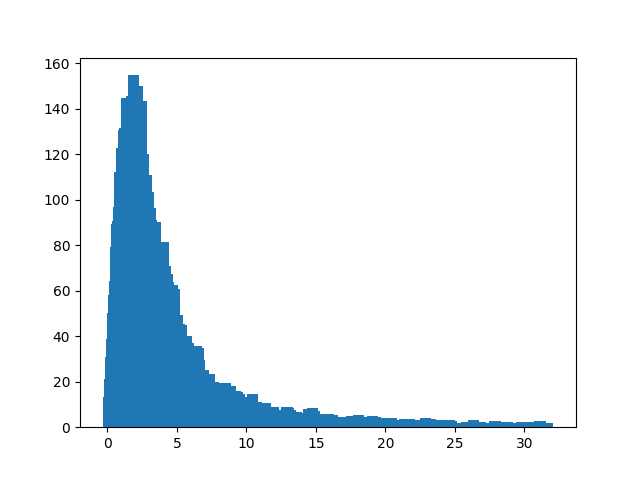
\includegraphics[scale=0.7]{diploma_results/static/ba_dist_beta_3.png}\\
\caption{Распределение индекса дружбы  в\\ стандартной модели Барабаши"---Альберт\\ при $m=3$}\label{fig:bas3}
\end{figure}

На Рис.\,\ref{fig:baps3} показан график распределения индекса дружбы в графе, построенном с помощью модифицированной модели Барабаши"---Альберт с параметром $ m=4 $. На основании этого графика можно сказать, что в данной модели выполняется парадокс дружбы.
\begin{figure}[!ht]
\centering
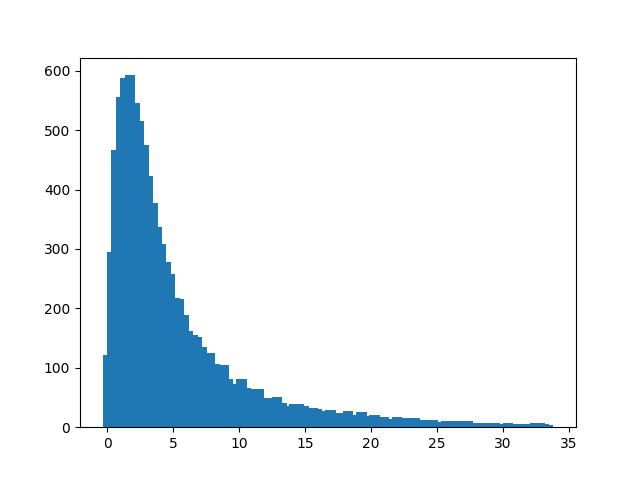
\includegraphics[scale=0.7]{diploma_results/static/bap_dist_beta_3.png}\\
\caption{Распределение индекса дружбы  в\\ модифицированной модели Барабаши"---Альберт\\ при $m=3$}\label{fig:baps3}
\end{figure}

График, на Рис.\,\ref{fig:triads3} показывает распределение индекса дружбы в графе, в основе которого лежит модель триадного замыкания. Этот график также подтверждает присутствие парадокса дружбы в рассматриваемой модели.
\begin{figure}[!ht]
\centering
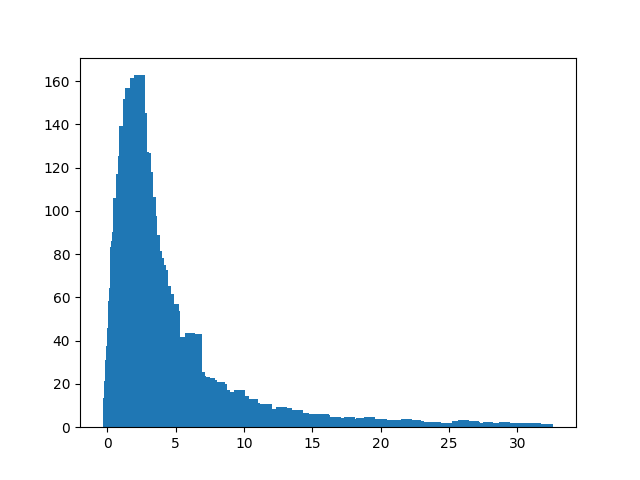
\includegraphics[scale=0.7]{diploma_results/static/triad_dist_beta_3_0.25.png}\\
\caption{Распределение индекса дружбы  в\\ модели триадного замыкания\\ при $m=3$ и $ p=0.25 $}\label{fig:triads3}
\end{figure}

На Рис.\,\ref{fig:basl3}, \ref{fig:bapsl3}, \ref{fig:triadsl3} выведены те же значения, но в логарифмической шкале. В соответствии с графиком, можно выдвинуть гипотезу, что распределение значений индекса дружбы происходит в соответствии со степенной функцией
\[
y = (\alpha \cdot x)^\gamma.
\]
\begin{figure}[!ht]
\centering
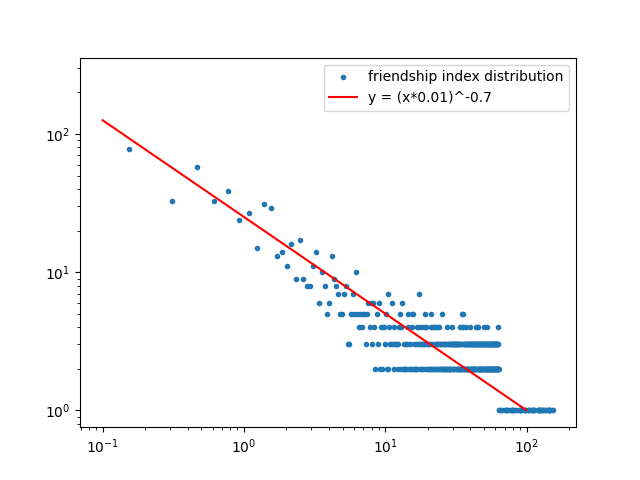
\includegraphics[scale=0.7]{diploma_results/static_log/ba_dist_beta_3.png}\\
\caption{Распределение индекса дружбы  в\\ стандартной модели Барабаши"---Альберт\\ при $m=3$, в логарифмической шкале}\label{fig:basl3}
\end{figure}
\begin{figure}[!ht]
\centering
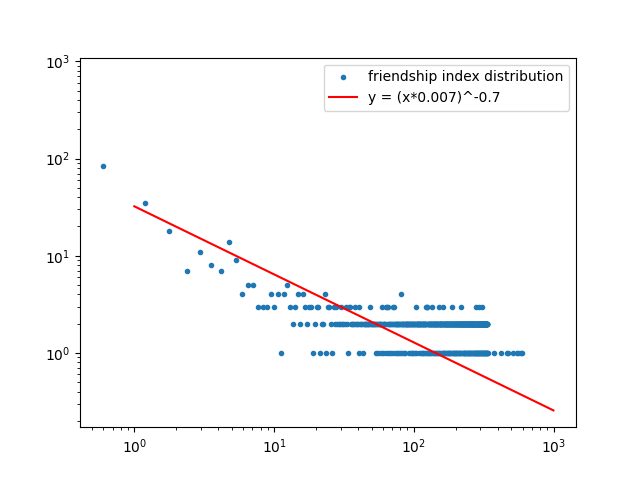
\includegraphics[scale=0.7]{diploma_results/static_log/bap_dist_beta_4.png}\\
\caption{Распределение индекса дружбы  в\\ модифицированной модели Барабаши"---Альберт\\ при $m=4$, в логарифмической шкале}\label{fig:bapsl3}
\end{figure}
\begin{figure}[!ht]
\centering
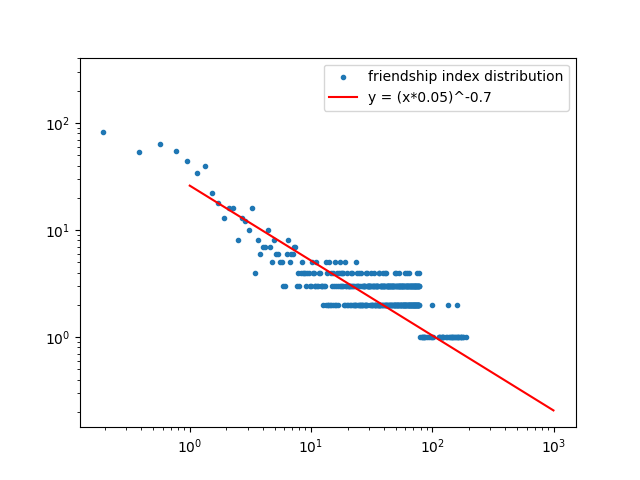
\includegraphics[scale=0.7]{diploma_results/static_log/triad_dist_beta_3_0.25.png}\\
\caption{Распределение индекса дружбы  в\\ модели триадного замыкания\\ при $m=3$ и $ p=0.25 $, в логарифмической шкале}\label{fig:triadsl3}
\end{figure}

Графики распределения индекса дружбы в этих моделях с другими параметрами $ m $ и $ p $ представлены в приложении~\ref{app:dist}.

Рисунок\,\ref{fig:badl3} содержит график в логарифмической шкале динамики среднего индекса дружбы в модели Барабаши"---Альберт при $m=3$ в сравнении с графиком степенной функции 
\[
y=(10000 \cdot x)^{0.12}.
\]
На основании данного графика можно сделать предположение, что среднее значение индекса дружбы в рассматриваемых моделях растёт в соответствии со степенной функцией. 
\begin{figure}[!ht]
\centering
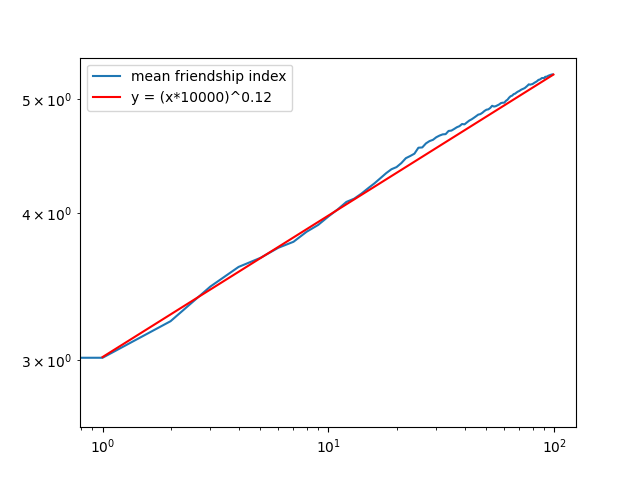
\includegraphics[scale=0.7]{diploma_results/dynamic_log/ba_mean_beta_3.png}\\
\caption{Динамика среднего значения индекса дружбы  в\\ стандартной модели Барабаши"---Альберт\\ при $m=3$, в логарифмической шкале}\label{fig:badl3}
\end{figure}

График динамики среднего индекса дружбы в модели Барабаши"---Альберт с пуассоновским распределением начальных степеней вершин при $m=4$ в логарифмической шкале, изображённый на Рис.\,\ref{fig:bapdl3}, совпадает с графиком степенной функции
\[
y=(80000 \cdot x)^{0.13}.
\]
\begin{figure}[!ht]
\centering
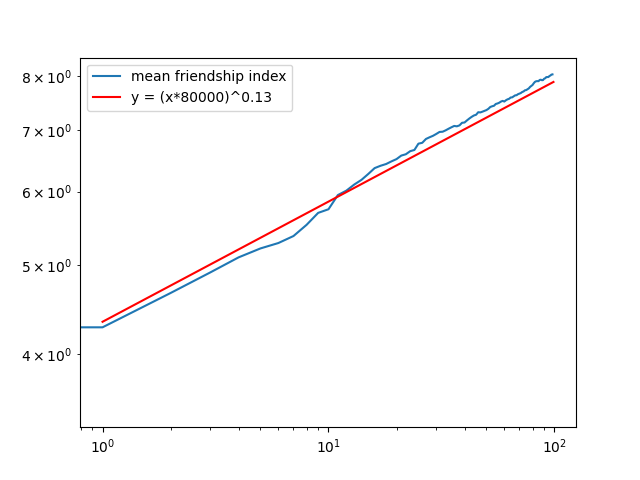
\includegraphics[scale=0.7]{diploma_results/dynamic_log/bap_mean_beta_4.png}\\
\caption{Динамика среднего значения индекса дружбы  в\\ модифицированной модели Барабаши"---Альберт\\ при $m=4$, в логарифмической шкале}\label{fig:bapdl3}
\end{figure}

На Рис.\,\ref{fig:triaddl3} показан график динамики среднего индекса дружбы в модели триадного замыкания при $m=3$ и $ p=0.25 $ в логарифмической шкале, который идентичен степенной функции:
\[
y=(40000 \cdot x)^{0.11}.
\]
\begin{figure}[!ht]
\centering
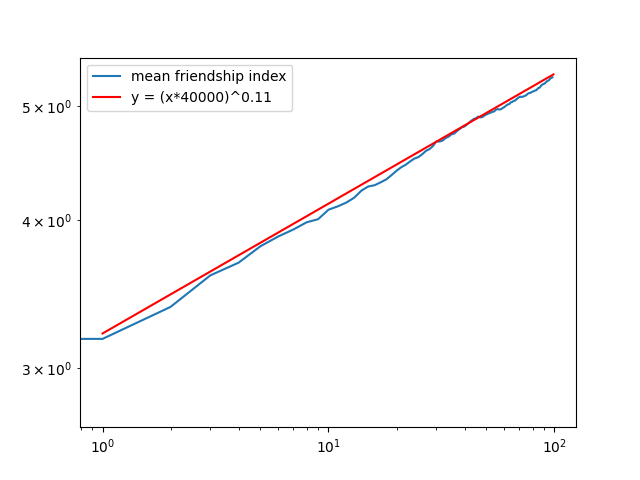
\includegraphics[scale=0.7]{diploma_results/dynamic_log/triad_mean_beta_3_0.25.png}\\
\caption{Динамика среднего значения индекса дружбы  в\\ модели триадного замыкания\\при $m=3$, в логарифмической шкале}\label{fig:triaddl3}
\end{figure}

Графики динамики индекса дружбы в других моделях представлены в приложении~\ref{app:dyn}.
\subsection{Анализ распределения и динамики индекса дружбы в реальных сетях}	
В ходе работы были рассмотрены графы следующих сетей из реального мира:
\begin{itemize}
\item LiveJournal
\item Twitter
\item Reddit
\item Google+
\item askubuntu
\item mathoverflow
\item superuser
\item сеть цитирования статей в сфере феноменология физики высоких энергий
\item внутренняя социальная сеть Калифорнийского университета в Ирвайне
\end{itemize}
\subsubsection{Анализ распределения индекса дружбы в социальной сети LiveJournal}
«Живой Журнал», «ЖЖ» (англ. LiveJournal, LJ) — блог-платформа для ведения онлайн-дневников (блогов), а также отдельный персональный блог, размещённый на этой платформе. Предоставляет возможность публиковать свои и комментировать чужие записи, вести коллективные блоги («сообщества»), добавлять в друзья («френдить») других пользователей и следить за их записями в «ленте друзей» («френдленте»). 

В работе рассматривался датасет сформированный на основе платформы «Живой Журнал» в 2009 годуи представленный в \cite{lj}. В графе в качестве вершин выступают пользователи, а наличие ребра между вершинами указывает на отношение дружбы между соответствующими пользователями. Граф содержит $4\,847\,571$ узлов и $68\,993\,773$ рёбер, что делает его слишком большим для рассмотрения динамики роста среднего индекса дружбы, но с другой стороны позволяет рассмотреть распределение индекса дружбы в крупном графе. 

На Рис. \ref{fig:lj} изображён график распределения индекса дружбы в описанном графе. Можно сделать предположение, что индекс дружбы распределён по степенному закону 
\[
y = (0.000002 \cdot x)^{-2}.
\]
Отметим, что схожесть со степенным законом распределения значений наблюдается так же и в графах, построенным в соответствии с моделями случайных графов, рассмотренных ранее в работе.

\begin{figure}[!ht]
\centering
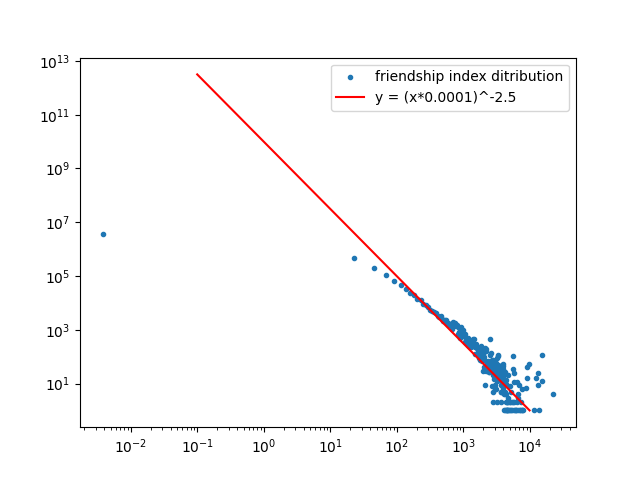
\includegraphics[scale=0.7]{diploma_results/static_real_log/soc-LiveJournal1.png}\\
\caption{Распределение индекса дружбы  в\\ социальной сети <<Живой Журнал>>\\ в логарифмической шкале}\label{fig:lj}
\end{figure}

\subsubsection{Анализ распределения индекса дружбы в социальной сети Twitter}
«Твиттер» (англ. Twitter, от англ. to tweet — «чирикать, щебетать, болтать») — американский сервис микроблогов и социальная сеть, в которой пользователи публикуют сообщения, известные как «твиты», и взаимодействуют с ними. Пользователи взаимодействуют с «Твиттером» через браузер, мобильное приложение или через API. До апреля 2020 года сервисы были доступны через SMS. Сервис предоставляется компанией Twitter, Inc., которая базируется в Сан-Франциско, Калифорния, и имеет более 26 офисов по всему миру.  В 2013 году он вошёл в десятку самых посещаемых сайтов и был назван «SMS интернета». К началу 2019 года у «Твиттера» было более 330 миллионов ежемесячных активных пользователей. На практике подавляющее большинство твитов пишет меньшинство пользователей. 

Данные об этой сети взяты из \cite{twit}. Граф описывает отношение дружбы между подтверждёнными пользователями, принадлежащим к определённым кругам таким как: <<деятели искусства>>, <<политики>> и т.д., он содержит $81\,306$ вершин связанных $1\,768\,149$ рёбрами. На графике, изображённом на Рис.\,\ref{fig:twit} можно обнаружить, что распределение индекса дружбы в данной сети мало соответствует степенной функции.

\begin{figure}[!ht]
\centering
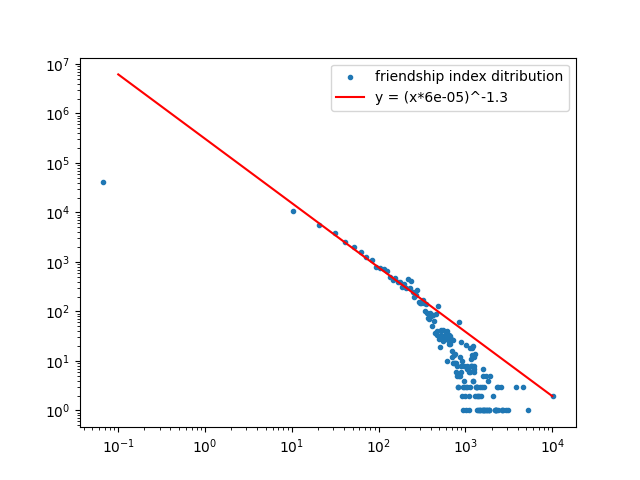
\includegraphics[scale=0.7]{diploma_results/static_real_log/twitter_combined.png}\\
\caption{Распределение индекса дружбы  в\\ социальной сети <<Twitter>>\\ в логарифмической шкале}\label{fig:twit}
\end{figure}

В данном графе также не удалось проанализировать динамику индекса дружбы.

\subsubsection{Анализ распределения и динамики индекса дружбы в сети цитирования статей в сфере феноменология физики высоких энергий}
Набор данных содержит информацию о $34\,546$ статьях на тему физики высоких энергий, опубликованных с января 1993 по апрель 2003 на arXiv.org "--- электронном архиве с открытым доступом для научных статей и препринтов по физике, математике, астрономии, информатике, биологии, электротехнике, статистике, финансовой математике и экономике. Граф содержит $421\,578$ рёбер. Датасет был представлен в работе \cite{cit}.

На Рис.\,\ref{fig:cits} изображено распределение индекса дружбы в данной сети. Из этого графика можно сделать предположение о том, что индекс дружбы в сети цитирования, как и индекс дружбы рассмотренных случайных графах, распределён по степенному закону 
\[
y = (0.0055 \cdot x)^{-2}
\].
\begin{figure}[!ht]
\centering
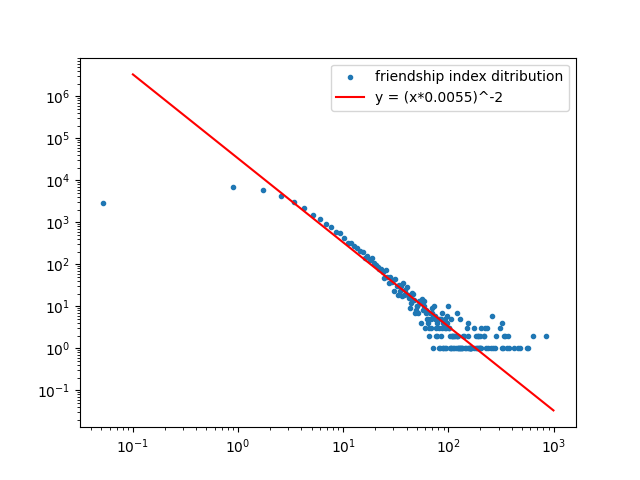
\includegraphics[scale=0.7]{diploma_results/static_real_log/Cit-HepPh.png}\\
\caption{Распределение индекса дружбы  в\\ сети цитирования\\ в логарифмической шкале}\label{fig:cits}
\end{figure}

График динамики индекса дружбы в данной сети представлен на Рис.\,\ref{fig:citd}. Можно выдвинуть гипотезу, что среднее значение индекса дружбы в графе растет в соответствии со степенной функцией 
\[
y = (11000 \cdot x)^{0.12}.
\]
Это, в части данного предположения, соответствует росту индекса дружбы в сетях моделей Барабаши"---Альберта и триадного замыкания.
\begin{figure}[!ht]
\centering
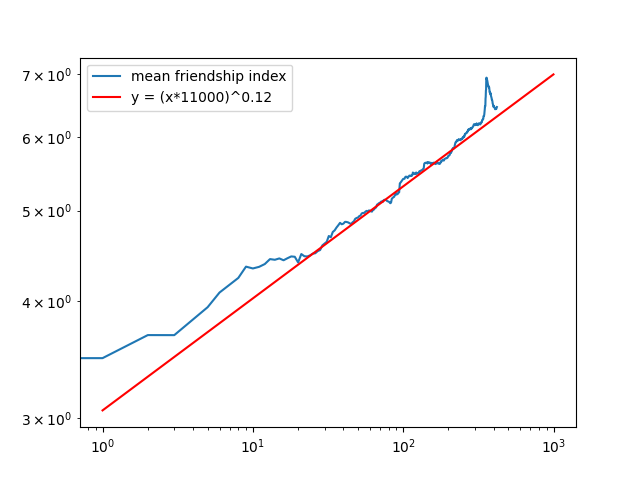
\includegraphics[scale=0.7]{diploma_results/dynamic_real_log/cit-HepPh_mean.png}\\
\caption{Динамика индекса дружбы  в\\ сети цитирования\\ в логарифмической шкале}\label{fig:citd}
\end{figure}

\subsubsection{Анализ распределения и динамики индекса дружбы в сети форума Reddit}
Reddit (рус. Реддит) — сайт, сочетающий черты социальной сети и форума, на котором зарегистрированные пользователи могут размещать ссылки на какую-либо понравившуюся информацию в интернете и обсуждать её. Как и многие другие подобные сайты, Reddit поддерживает систему голосования за понравившиеся сообщения — наиболее популярные из них оказываются на заглавной странице сайта. Один из наиболее популярных сайтов в мире — 20-е место по посещаемости по данным SimilarWeb. 

В данном случае рассматривается сеть гиперссылок между субредитами (сообществами на <<Reddit>>) данные собирались на протяжении двух с половиной лет: с января 2014 по апрель 2017. Граф состоит из $55\,863$ узлов, соединённых $858\,490$ рёбрами. Данные были представлены в \cite{reddit}.

На Рис.\,\ref{fig:reds} представлен график распределения индекса дружбы в графе гиперссылок между субредитами. По графику можно сделать предположение, что распределение индекса дружбы в данной сети также соответствует степенной функции, которая в данном случае выглядит следующим образом:
\[
y = (2e^{-6} \cdot x)^{-1}.
\]
\begin{figure}[!ht]
\centering
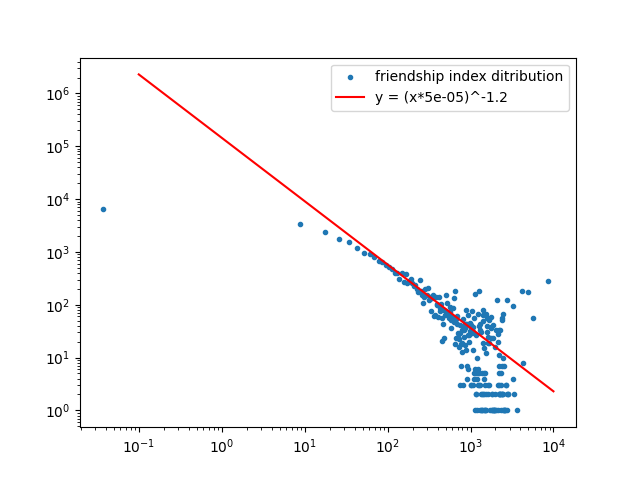
\includegraphics[scale=0.7]{diploma_results/static_real_log/soc-redditHyperlinks-body.png}\\
\caption{Распределение индекса дружбы  в\\ сети форума Reddit\\ в логарифмической шкале}\label{fig:reds}
\end{figure}

Рис.\,\ref{fig:redd} указывает на сходство графика динамики индекса дружбы на форуме Reddit, с графиком степенной функции 
\[
y = (0.03 \cdot x)^{0.8}.
\]
\begin{figure}[!ht]
\centering
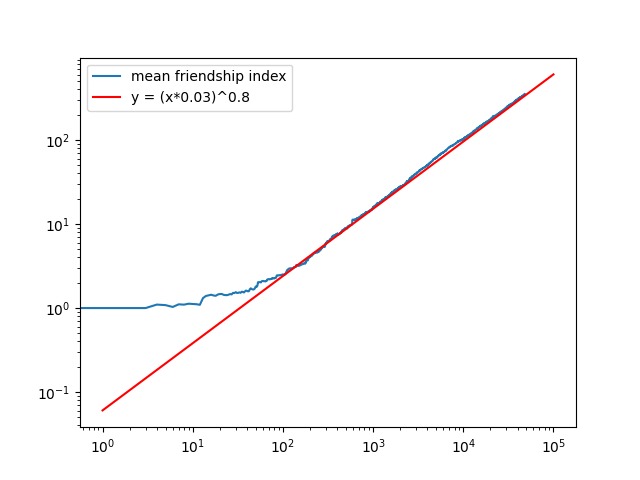
\includegraphics[scale=0.7]{diploma_results/dynamic_real_log/soc-redditHyperlinks-body_mean.png}\\
\caption{Динамика индекса дружбы  в\\ сети форума Reddit\\ в логарифмической шкале}\label{fig:redd}
\end{figure}

\subsubsection{Анализ распределения и динамики индекса дружбы в системе вопросов и ответов AskUbuntu}
AskUbuntu "--- веб-сайт для работы с вопросами и ответами возникающими при использовании дистрибутива Linux Ubuntu. Сайты позволяют пользователям задавать вопросы и отвечать на них. Путём учёта активной деятельности, происходит голосование за вопросы и ответы, положительное и отрицательное. Редактировать вопросы и ответы возможно в вики-режиме. Все материалы, публикуемые в сети, доступны под свободной лицензией CC BY-SA. 

Были рассмотрены 4 датасета: 
\begin{itemize}
\item граф ответов на вопросы, который состоит из $137,517$ вершин, представляющих пользователей, и $280\,102$ связей между ними, связь между пользователями $A$ и $B$ заключается в том, что пользователь $A$ ответил на вопрос пользователя $B$;
\item граф цитирования вопросов, содержащий $79\,155$ узлов и $327\,513$ рёбер, где направленное ребро проводится между пользователем и автором вопроса, который он процитировал;
\item граф цитирования ответов из $75\,555$ и $356\,822$ вершин и рёбер, соответственно, ребро проводится от пользователя сославшегося на ответ к пользователю его написавшему;
\item и общий граф содержащий всех пользователей и все рёбра всех предыдущих графов, в нём $159\,316$ узлов и $964,437$ связей.
\end{itemize}
Данные для этих графов собирались на протяжении более чем семи лет, они были представлены в статье \cite{au}.

Свойства данной сети не полностью соответствуют поведению, изучаемых в дипломной работе моделей: на Рис.\,\ref{fig:aus} можно увидеть, что распределение индекса дружбы плохо соответствует степенной функции и, следовательно, не соответствует построенным моделям.

\begin{figure}[!ht]
\centering
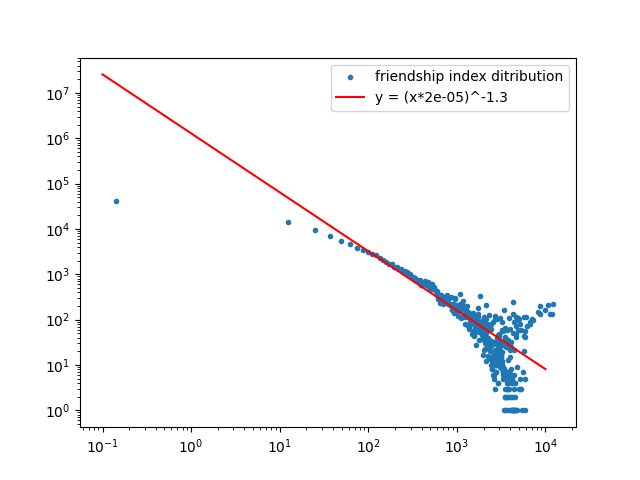
\includegraphics[scale=0.7]{diploma_results/static_real_log/sx-askubuntu.png}\\
\caption{Распределение индекса дружбы  в\\ сети AskUbuntu\\ в логарифмической шкале}\label{fig:aus}
\end{figure}

Однако, среднее значение индекса дружбы, как и в моделях случайных графов, растёт скорее по степенному закону 
\[
y = (0.8 \cdot x)^{0.5},
\]
что показано на графике \ref{fig:aud}.
\begin{figure}[!ht]
\centering
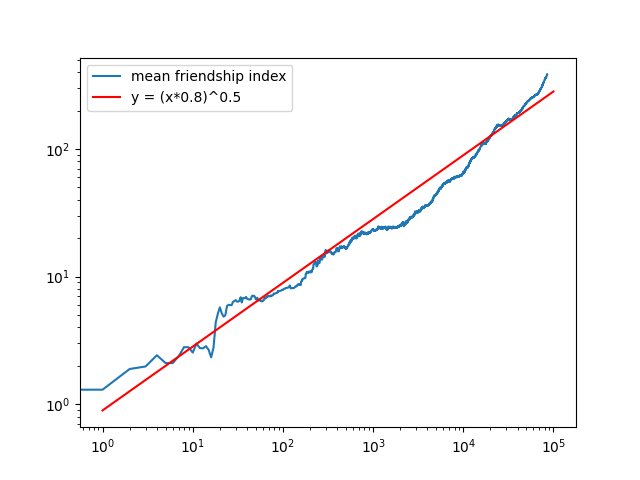
\includegraphics[scale=0.7]{diploma_results/dynamic_real_log/sx-askubuntu_mean.png}\\
\caption{Динамика индекса дружбы  в\\ сети askubuntu\\ в логарифмической шкале}\label{fig:aud}
\end{figure}

Наиболее ярко данные закономерности проявляются в графе сети ответов на вопросы, графики распределения и динамики индекса дружбы в которой изображены на Рис.\,\ref{fig:auaqs} и \ref{fig:auaqd}, соответственно.

\begin{figure}[!ht]
\centering
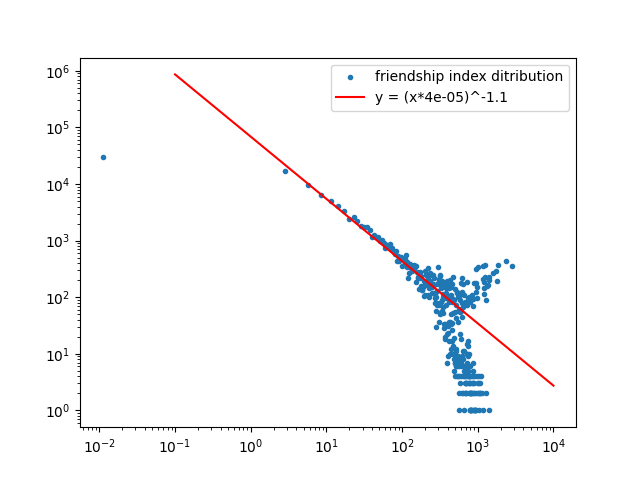
\includegraphics[scale=0.7]{diploma_results/static_real_log/sx-askubuntu-a2q.png}\\
\caption{Распределение индекса дружбы  в\\ сети ответов на вопросы на AskUbuntu\\ в логарифмической шкале}\label{fig:auaqs}
\end{figure}

\begin{figure}[!ht]
\centering
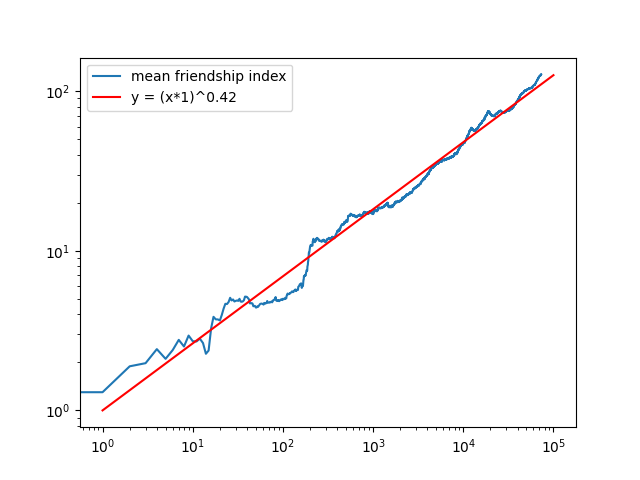
\includegraphics[scale=0.7]{diploma_results/dynamic_real_log/sx-askubuntu-a2q_mean.png}\\
\caption{Динамика индекса дружбы  в\\ сети ответов на вопросы на AskUbuntu\\ в логарифмической шкале}\label{fig:auaqd}
\end{figure}

Графики других подсетей представлены в приложении~\ref{app:real}

\subsubsection{Анализ распределения и динамики индекса дружбы в системе вопросов и ответов SuperUser}
SuperUser также как и AskUbuntu является платформой вопросов и ответов, в отличии от предыдущей сети она посвящена компьютерным энтузиастам. Как и AskUbuntu она выступает в качестве одного из разделов StackExchange и она подчиняется тем же базовым правилам сети: любой пользователь может задать вопрос, любой может на него ответить и любой может проголосовать за ответ или вопрос.

Для этой сети были выделены также три подсети:
\begin{itemize}
\item сеть ответов на вопросы
\item сеть цитирования вопросов
\item сеть цитирования ответов
\end{itemize}
Данные были также представлены в работе \cite{au}.

Сеть платформы SuperUser не подчиняется закономерностям выявленным в случайных графах в ходе данной работы. На Рис.\,\ref{fig:sus} можно увидеть, что график распределения индекса дружбы скорее плохо совпадает со степенной функцией, также как и график динамики индекса дружбы представленный на Рис.\,\ref{fig:sud}.
\begin{figure}[!ht]
\centering
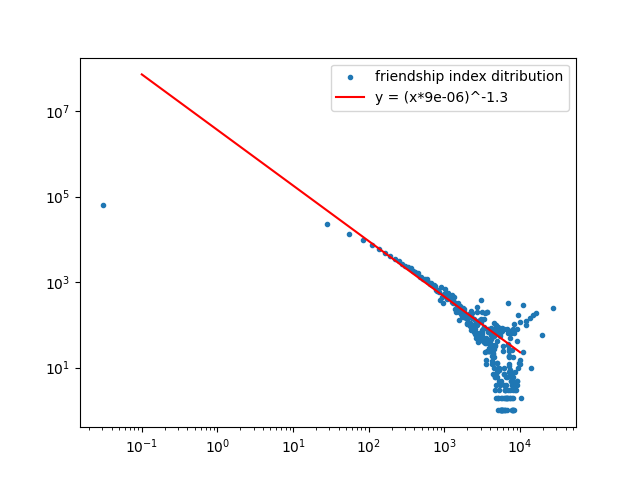
\includegraphics[scale=0.7]{diploma_results/static_real_log/sx-superuser.png}\\
\caption{Распределение индекса дружбы  в\\ сети SuperUser\\ в логарифмической шкале}\label{fig:sus}
\end{figure}
\begin{figure}[!ht]
\centering
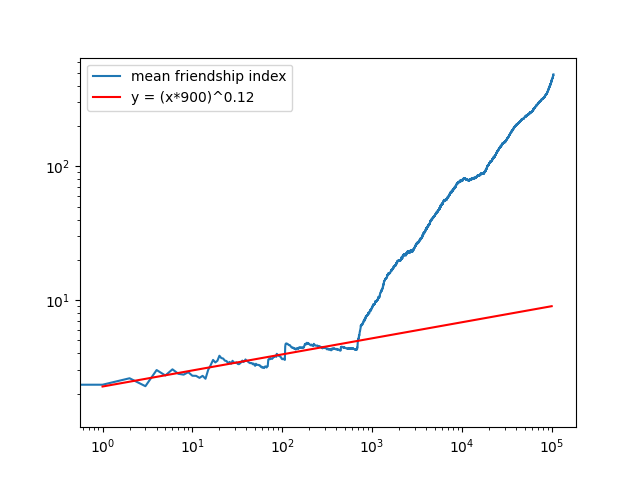
\includegraphics[scale=0.7]{diploma_results/dynamic_real_log/sx-superuser_mean.png}\\
\caption{Динамика индекса дружбы  в\\ сети SuperUser\\ в логарифмической шкале}\label{fig:sud}
\end{figure}

В сети цитирования вопросов это отклонение только усиливается, что можно наблюдать на графиках \ref{fig:sucqs} и \ref{fig:sucqd}.
\begin{figure}[!ht]
\centering
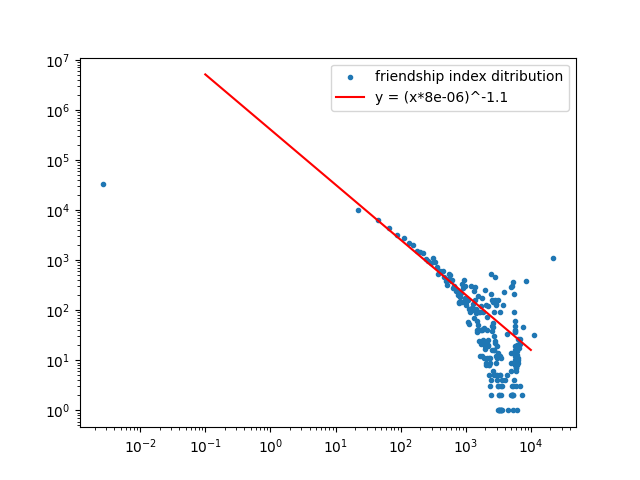
\includegraphics[scale=0.7]{diploma_results/static_real_log/sx-superuser-c2q.png}\\
\caption{Распределение индекса дружбы  в\\ сети цитирования вопросов на SuperUser\\ в логарифмической шкале}\label{fig:sucqs}
\end{figure}
\begin{figure}[!ht]
\centering
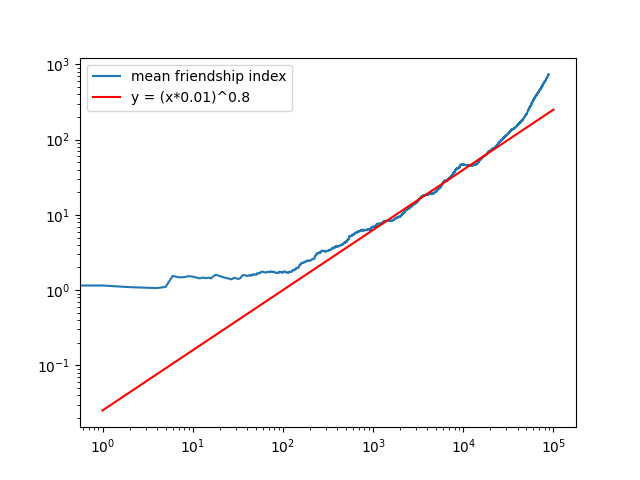
\includegraphics[scale=0.7]{diploma_results/dynamic_real_log/sx-superuser-c2q_mean.png}\\
\caption{Динамика индекса дружбы  в\\ сети цитирования вопросов на SuperUser\\ в логарифмической шкале}\label{fig:sucqd}
\end{figure}

В то же время, в подсети ответов на вопросы динамика индекса дружбы всё же, вероятно, подчиняется степенному закону, что можно наблюдать на Рис.\,\ref{fig:suaqd}.
\begin{figure}[!ht]
\centering
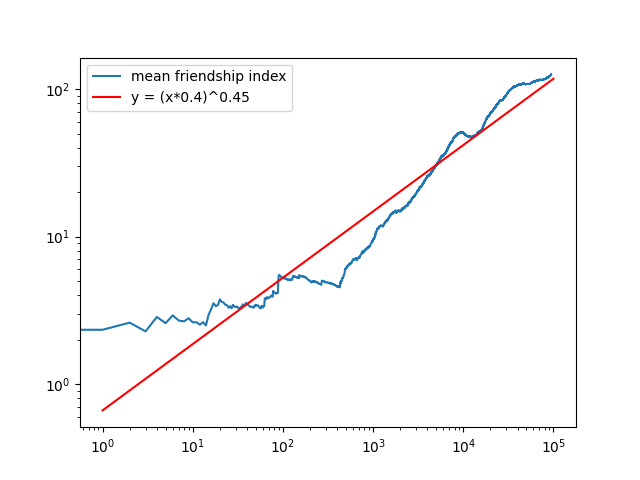
\includegraphics[scale=0.7]{diploma_results/dynamic_real_log/sx-superuser-a2q_mean.png}\\
\caption{Динамика индекса дружбы  в\\ сети ответов на вопросы на SuperUser\\ в логарифмической шкале}\label{fig:suaqd}
\end{figure}

Графики для оставшихся подсетей представлены в приложении \ref{app:real}, там же расположены графики распределения и динамики индекса дружбы в сетях Google+, mathoverflow и сети сообщений студентов Калифорнийского университета в Ирвайне, данные для которых были взяты из работ \cite{twit}, \cite{au} и \cite{stdmsg}. В таблице\ref{tab:general} представлен сравнительный анализ всех рассмотренных сетей.
\begin{table}[!ht]
\small
\caption{Сводная таблица результатов экспериментов}\label{tab:general}
\begin{tabular}{>{\raggedright}p{7cm}@{\ }>{\centering}p{3cm}@{\ }>{\centering}p{1.1cm}@{\ }>{\centering}p{3cm}@{\ }>{\centering}p{1cm}}
\hline\noalign{\smallskip}
\centering Сеть & Функция распределения индекса дружбы & $\gamma_{ dist }$ & Функция динамики индекса дружбы & $\gamma_{ dyn }$\cr 
\noalign{\smallskip}\hline\noalign{\smallskip}
Модель Барабаши"---Альберт при $m=3$&степенная&-0.7&степенная&0.15\cr 
Модель Барабаши"---Альберт при $m=3$&степенная&-0.7&степенная&0.15\cr 
Модель Барабаши"---Альберт с пуассоновским распределением начальных степеней при $m=4$&степенная&-0.5&степенная&0.15\cr 
Модель Барабаши"---Альберт с пуассоновским распределением начальных степеней при $m=5$&степенная&-0.5&степенная&0.15\cr 
Модель Барабаши"---Альберт с пуассоновским распределением начальных степеней при $m=6$&степенная&-0.45&степенная&0.15\cr 
Модель триадного замыкания при $m=3$ и $p=0.25$&степенная&-0.7&степенная&0.15\cr 
Модель триадного замыкания при $m=3$ и $p=0.5$&степенная&-0.7&степенная&0.15\cr 
Модель триадного замыкания при $m=3$ и $p=0.75$&степенная&-0.4&степенная&0.12\cr 
Модель триадного замыкания при $m=5$ и $p=0.25$&степенная&-0.6&степенная&0.13\cr 
Модель триадного замыкания при $m=5$ и $p=0.5$&степенная&-0.6&степенная&0.13\cr 
Модель триадного замыкания при $m=5$ и $p=0.75$&степенная&-0.55&степенная&0.12\cr \cr
Twitter&неизвес"-тная функция&N/A&N/A&N/A\cr 
Google+&степенная&-1.7&N/A&N/A\cr 
Reddit&степенная&-1.2&степенная&0.8\cr 
AskUbuntu&неизвес"-тная функция&N/A&степенная&0.5\cr 
MathOverflow&степенная&-1.2&степенная&0.45\cr 
SuperUser&неизвес"-тная функция&N/A&экспонен"-циальная&N/A\cr 
Сеть цитирования&степенная&-2&степенная&0.12\cr 
LiveJournal&степенная&-2.5&N/A&N/A\cr 
Сеть студенческих сообщений&степенная&-0.9&степенная&0.5\cr 
\noalign{\smallskip}\hline
\end{tabular}
\end{table}

% Раздел "Заключение"
\conclusion
В ходе выполнения дипломной работы были изучены различные модели генерации растущих сетей. Были реализованы модели построения случайных графов:
\begin{itemize}
\item стандартная модель Барабаши"--~Альберт; 
\item модель Барабаши"--~Альберт с пуассоновским распределением начальных степеней узлов; 
\item модель триадного замыкания.
\end{itemize} 

В соответствии с реализованными моделями проведена серия экспериментов в которых строились случайные графы и исследовались динамика среднего значения индекса дружбы в сети и распределение значений индекса дружбы в итоговом графе. В соответствии полученными результатами выдвинута гипотеза, что распределение индекса дружбы вершин итогового графа и рост среднего значения индекса дружбы в ходе формирования сети происходит по степенному закону.  

Были исследованы значения распределения индекса дружбы и динамики роста среднего значения индекса дружбы в ряде реальных сетей. Сделан вывод, что для большинства сетей поведение индекса дружбы схоже с его поведением в сетях растущих по исследуемым моделям.

Реализация моделей и эксперименты проводились на языке python  с использованием библиотек json, multiprocessing, pyplot, numpy, random.


% Список литературы
\bibliographystyle{gost780uv}
\bibliography{thesis}

% Окончание основного документа и начало приложений
% Каждая последующая секция документа будет являться приложением

\appendix
\section{Текст программы}\label{app:program}
В этом приложении приведён полный текст реализации модели Барабаши"--~Альберт.
\begin{minted}{python}
from multiprocessing.dummy import current_process
from statistics import mean

import matplotlib as mpl
import matplotlib.pyplot as plt
import math
import random
import pylab
import multiprocessing
import datetime
import numpy as np
import json

def my_bag_poisson(n, args, funcs, dts):
    m = args[0]
    ans = [[] for _ in range(len(dts))]
    m0 = np.random.poisson(m)
    degrees = list(np.full(m0 + 1, m0))
    neibours = [list(np.delete(np.arange(m0 + 1), i)) for i in np.arange(m0 + 1)]
    nodes = np.arange(m0 + 1)
    used = np.full(n, False)
    for i in range(m0, n):
        mi = max(1, min(np.random.poisson(m), nodes.shape[0]))
        conections = []
        j = 0
        while j < mi:
            choosen = random.choices(nodes, weights = degrees, k = 1)[0]
            if not used[choosen]:
                j += 1
                conections.append(choosen)
                used[choosen] = True
        neibours.append([])
        for j in conections:
            used[j] = False
            neibours[i + 1].append(j)
            neibours[j].append(i)
            degrees[j] += 1
        degrees.append(mi)
        nodes = np.append(nodes, nodes.shape[0])
        for j in range(len(dts)):
            if i % dts[j] == 0:
                ans[j].append(funcs[j](degrees, neibours))
    return ans

def my_triad(n, args, funcs, dts):
    m = args[0]
    p = args[1]
    ans = [[] for _ in range(len(dts))]
    degrees = list(np.full(m + 1, m))
    neibours = [list(np.delete(np.arange(m + 1), i)) for i in np.arange(m + 1)]
    nodes = np.arange(m + 1)
    used = np.full(n, False)
    for i in range(m, n):
        conections = []
        j = 0
        while j < m:
            if j == 0 or np.random.rand() > p:
                choosen = random.choices(nodes, weights = degrees, k = 1)[0]
            else:
                choosen = random.choices(neibours[conections[0]], k = 1)[0]
            if not used[choosen]:
                j += 1
                conections.append(choosen)
                used[choosen] = True
        neibours.append([])
        for j in conections:
            used[j] = False
            neibours[i + 1].append(j)
            neibours[j].append(i)
            degrees[j] += 1
        degrees.append(m)
        nodes = np.append(nodes, nodes.shape[0])
        for j in range(len(dts)):
            if i % dts[j] == 0:
                ans[j].append(funcs[j](degrees, neibours))
    return ans


def my_bag(n, args, funcs, dts):
    m = args[0]
    ans = [[] for _ in range(len(dts))]
    degrees = list(np.full(m + 1, m))
    neibours = [list(np.delete(np.arange(m + 1), i)) for i in np.arange(m + 1)]
    nodes = np.arange(m + 1)
    used = np.full(n, False)
    for i in range(m, n):
        conections = []
        j = 0
        while j < m:
            choosen = random.choices(nodes, weights = degrees, k = 1)[0]
            if not used[choosen]:
                j += 1
                conections.append(choosen)
                used[choosen] = True
        neibours.append([])
        for j in conections:
            used[j] = False
            neibours[i + 1].append(j)
            neibours[j].append(i)
            degrees[j] += 1
        degrees.append(m)
        nodes = np.append(nodes, nodes.shape[0])
        for j in range(len(dts)):
            if i % dts[j] == 0:
                ans[j].append(funcs[j](degrees, neibours))
    return ans

def run_thread(N, i, res, model, n, args, funcs, dts):
    ans = []
    for j in range(N):
        ans.append(model(n, args, funcs, dts))
    res[i] = ans
def run(N, treads, model, n, args, funcs, dts):
    procs = []
    manager = multiprocessing.Manager()
    res = manager.dict()
    for i in range(treads):
        curn = min(N, math.ceil(N / (treads - i)))
        p = multiprocessing.Process(target=run_thread, args=(curn, i, res, model, n, args, funcs, dts))
        N -= curn
        procs.append(p)
        p.start()
    for proc in procs:
        proc.join()
    ans = []
    for i in res.values():
        ans += i
    return ans
def d (degrees, neibours):
    return degrees
def neibours (degrees, neibours):
    return neibours
def index (degrees, neibours):
    return np.arange(len(neibours))
def s (degrees, neibours):
    return [sum([degrees[i] for i in j]) for j in neibours]
def alfa (degrees, neibours):
    return [si / di for (si, di) in zip(s(degrees, neibours), d(degrees, neibours))]
def beta (degrees, neibours):
    return [ai / di for (ai, di) in zip(alfa(degrees, neibours), d(degrees, neibours))]
def mean_beta (degrees, neibours):
    return [mean(beta(degrees, neibours))]

if __name__ == "__main__":
    n = 100000
    m = 5
    p = 0.25
    
    for m in [3, 5]:
        for p in [0.25, 0.5, 0.75]:
            ans = run(1, 6, my_triad, n, [m, p], [index, d, neibours], [n - 1, n - 1, n - 1])
            ans = ans[0]
            ans = [i[0] for i in ans]
            prejson = [{'index':int(ans[0][i]), 'degree':int(ans[1][i]), 'neibours':[int(j) for j in ans[2][i]]} for i in range(len(ans[0]))]
            with open('\\source\\repos\\CSW\\diploma_results\\triad_graph_' + str(m) + '_' + str(p) + '.json', 'w') as f:
                json.dump(prejson, f)
                f.close()
    
    for m in [4, 5, 6]:
        ans = run(10, 6, my_bag_poisson, n, [m, p], [index, d, neibours], [n - 1, n - 1, n - 1])
        ans = ans[0]
        ans = [i[0] for i in ans]
        prejson = [{'index':int(ans[0][i]), 'degree':int(ans[1][i]), 'neibours':[int(j) for j in ans[2][i]]} for i in range(len(ans[0]))]
        with open('\\source\\repos\\CSW\\diploma_results\\bap_graph_' + str(m) + '.json', 'w') as f:
            json.dump(prejson, f)
            f.close()
            
    
    for m in [3, 5]:
        ans = run(1, 6, my_bag, n, [m, p], [index, d, neibours], [n - 1, n - 1, n - 1])
        ans = ans[0]
        ans = [i[0] for i in ans]
        prejson = [{'index':int(ans[0][i]), 'degree':int(ans[1][i]), 'neibours':[int(j) for j in ans[2][i]]} for i in range(len(ans[0]))]
        with open('\\source\\repos\\CSW\\diploma_results\\ba_graph_' + str(m) + '.json', 'w') as f:
            json.dump(prejson, f)
            f.close()
            
        
    for m in [4, 6]:
        ans = run(1, 6, my_bag_poisson, n, [m], [mean_beta], [100])
        mean_beta_data = np.array([i[0] for i in ans])
        mean_beta_data = np.apply_along_axis(arr=mean_beta_data, axis=2, func1d=lambda x: x[0])
        mean_beta_data = mean_beta_data.transpose((1, 0))
        mean_beta_data = np.apply_along_axis(arr=mean_beta_data, axis=1, func1d=mean)
        plt.plot(np.arange(mean_beta_data.shape[0]), mean_beta_data)
        plt.savefig('\\source\\repos\\CSW\\diploma_results\\bap_mean_beta_' + str(m) + '.jpg')
        plt.clf()
            
    
    for m in [3]:
        ans = run(10, 6, my_bag, n, [m], [mean_beta], [100])
        mean_beta_data = np.array([i[0] for i in ans])
        mean_beta_data = np.apply_along_axis(arr=mean_beta_data, axis=2, func1d=lambda x: x[0])
        mean_beta_data = mean_beta_data.transpose((1, 0))
        mean_beta_data = np.apply_along_axis(arr=mean_beta_data, axis=1, func1d=mean)
        plt.plot(np.arange(mean_beta_data.shape[0]), mean_beta_data)
        plt.savefig('\\source\\repos\\CSW\\diploma_results\\ba_mean_beta_' + str(m) + '.jpg')
        plt.clf()
\end{minted}
\section{Графики распределения индекса дружбы в построенных графах}\label{app:dist}
\begin{figure}[!ht]
    \centering
    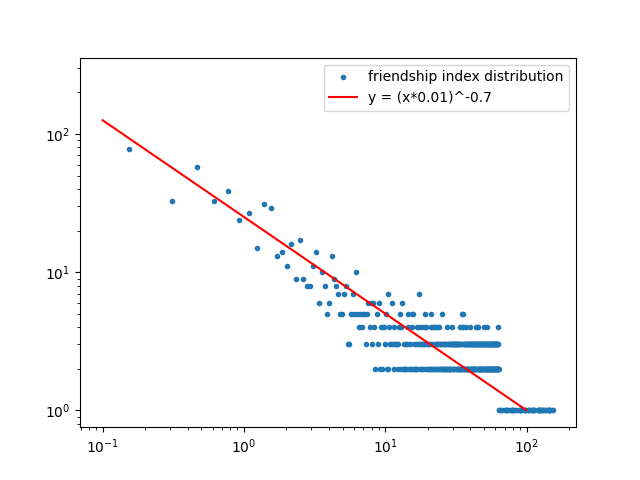
\includegraphics[scale=0.5]{diploma_results/static_log/ba_dist_beta_3.png}
    \caption{Распределение индекса дружбы  в\\ модели Барабаши"---Альберт\\ при $m=3$}
\end{figure}
\begin{figure}[!ht]
    \centering
    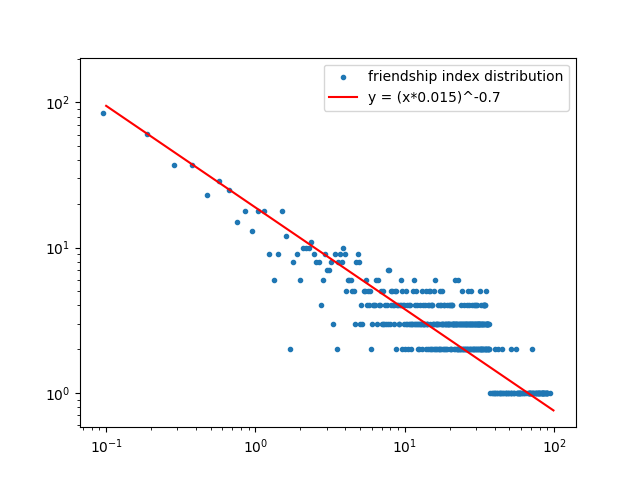
\includegraphics[scale=0.5]{diploma_results/static_log/ba_dist_beta_5.png}
    \caption{Распределение индекса дружбы  в\\ модели Барабаши"---Альберт\\ при $m=5$}
\end{figure}
\begin{figure}[!ht]
    \centering
    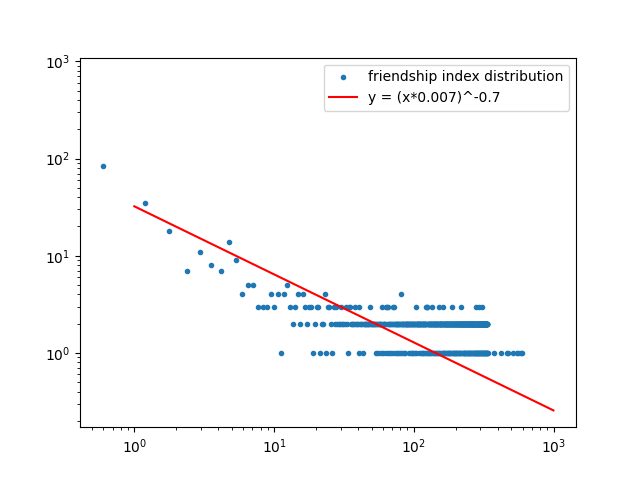
\includegraphics[scale=0.5]{diploma_results/static_log/bap_dist_beta_4.png}
    \caption{Распределение индекса дружбы  в\\ модели Барабаши"---Альберт\\ с пуассоновским распределением\\ степеней новых вершин \\ при $\lambda=4$}
\end{figure}
\begin{figure}[!ht]
    \centering
    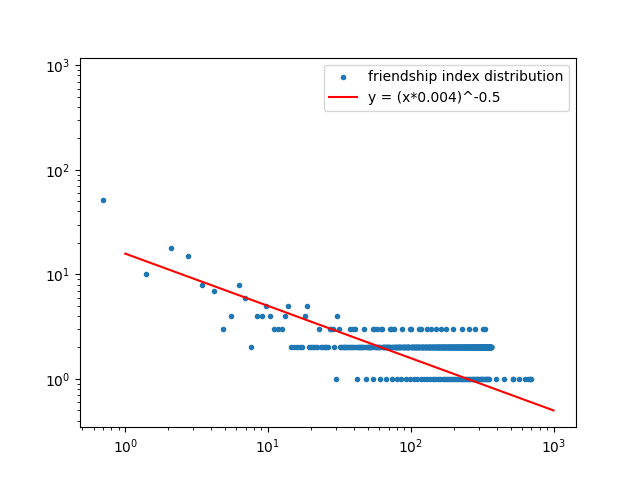
\includegraphics[scale=0.5]{diploma_results/static_log/bap_dist_beta_5.png}
        \caption{Распределение индекса дружбы  в\\ модели Барабаши"---Альберт\\ с пуассоновским распределением\\ степеней новых вершин \\ при $\lambda=5$}
\end{figure}
\begin{figure}[!ht]
    \centering
    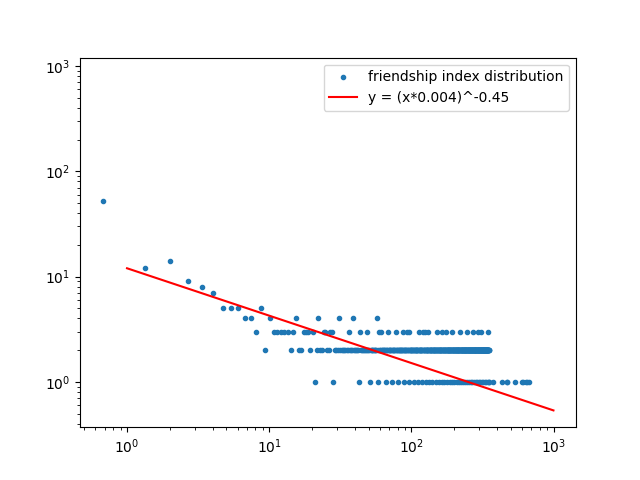
\includegraphics[scale=0.5]{diploma_results/static_log/bap_dist_beta_6.png}
        \caption{Распределение индекса дружбы  в\\ модели Барабаши"---Альберт\\ с пуассоновским распределением\\ степеней новых вершин \\ при $\lambda=6$}
\end{figure}
\begin{figure}[!ht]
    \centering
    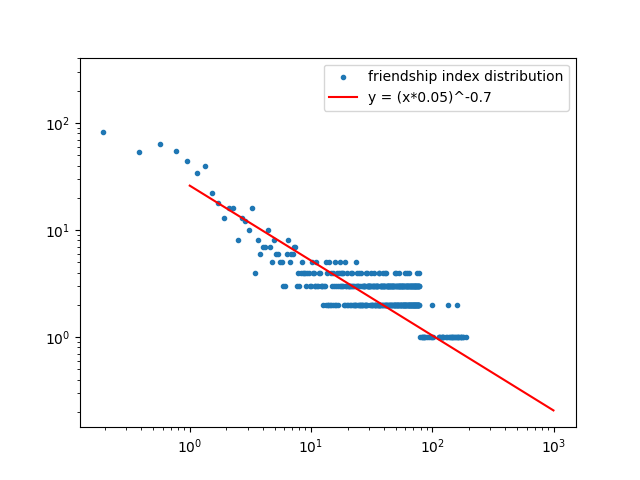
\includegraphics[scale=0.5]{diploma_results/static_log/triad_dist_beta_3_0.25.png}
    \caption{Распределение индекса дружбы  в\\ модели триадного замыкания\\ при $m=3$ и $p=0.25$}
\end{figure}
\begin{figure}[!ht]
    \centering
    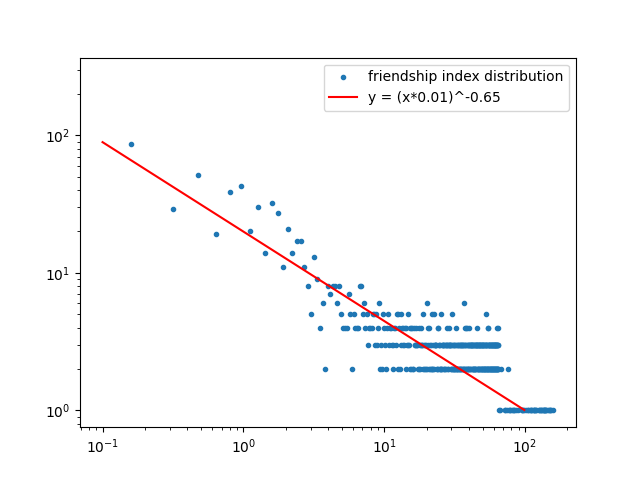
\includegraphics[scale=0.5]{diploma_results/static_log/triad_dist_beta_3_0.5.png}
    \caption{Распределение индекса дружбы  в\\ модели триадного замыкания\\ при $m=3$ и $p=0.5$}
\end{figure}
\begin{figure}[!ht]
    \centering
    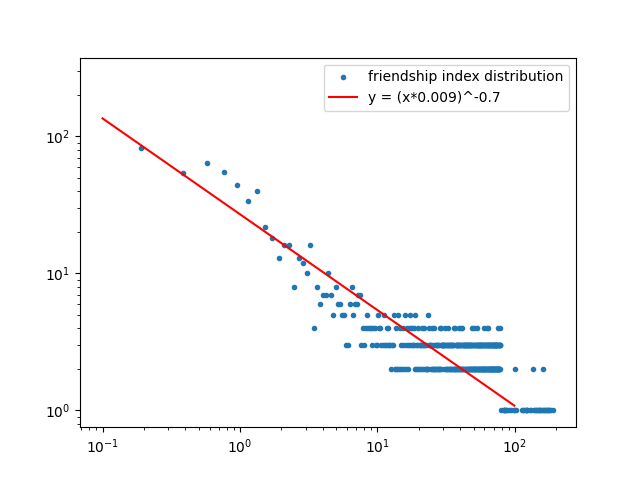
\includegraphics[scale=0.5]{diploma_results/static_log/triad_dist_beta_3_0.75.png}
    \caption{Распределение индекса дружбы  в\\ модели триадного замыкания\\ при $m=3$ и $p=0.75$}
\end{figure}
\begin{figure}[!ht]
    \centering
    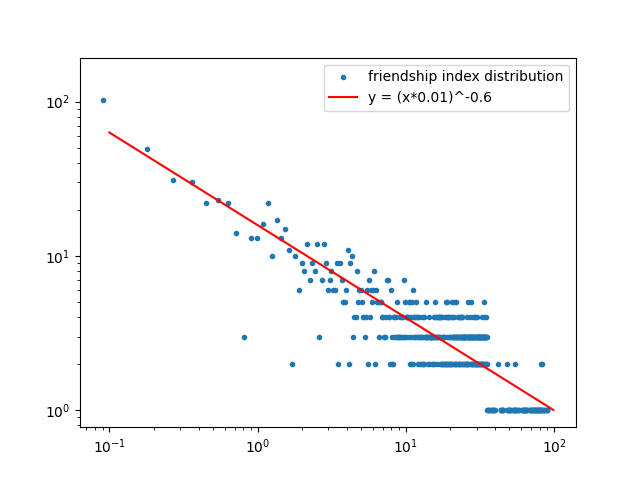
\includegraphics[scale=0.5]{diploma_results/static_log/triad_dist_beta_5_0.25.png}
    \caption{Распределение индекса дружбы  в\\ модели триадного замыкания\\ при $m=5$ и $p=0.25$}
\end{figure}
\begin{figure}[!ht]
    \centering
    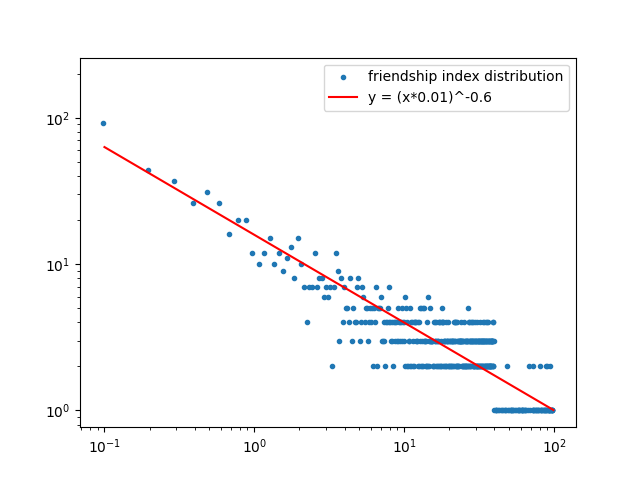
\includegraphics[scale=0.5]{diploma_results/static_log/triad_dist_beta_5_0.5.png}
    \caption{Распределение индекса дружбы  в\\ модели триадного замыкания\\ при $m=5$ и $p=0.5$}
\end{figure}
\begin{figure}[!ht]
    \centering
    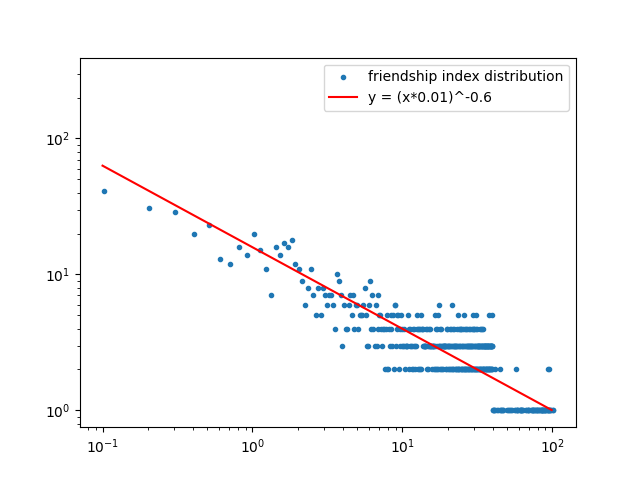
\includegraphics[scale=0.7]{diploma_results/static_log/triad_dist_beta_5_0.75.png}
    \caption{Распределение индекса дружбы  в\\ модели триадного замыкания\\ при $m=5$ и $p=0.75$}
\end{figure}
\section{Графики динамики среднего индекса дружбы в построенных графах}\label{app:dyn}
\begin{figure}[!ht]
    \centering
    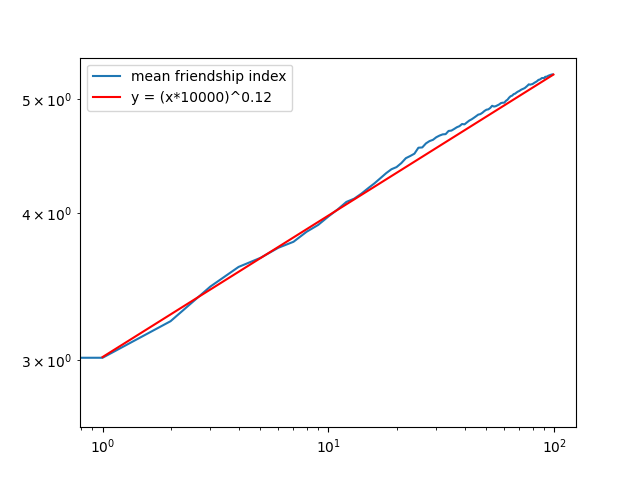
\includegraphics[scale=0.7]{diploma_results/dynamic_log/ba_mean_beta_3.png}
    \caption{Динамика среднего индекса дружбы  в\\ модели Барабаши"---Альберт\\ при $m=3$}
\end{figure}
\begin{figure}[!ht]
    \centering
    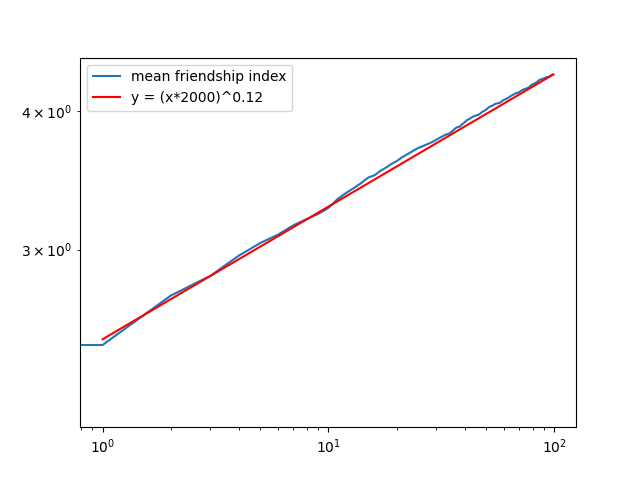
\includegraphics[scale=0.7]{diploma_results/dynamic_log/ba_mean_beta_5.png}
    \caption{Динамика среднего индекса дружбы  в\\ модели Барабаши"---Альберт\\ при $m=5$}
\end{figure}
\begin{figure}[!ht]
    \centering
    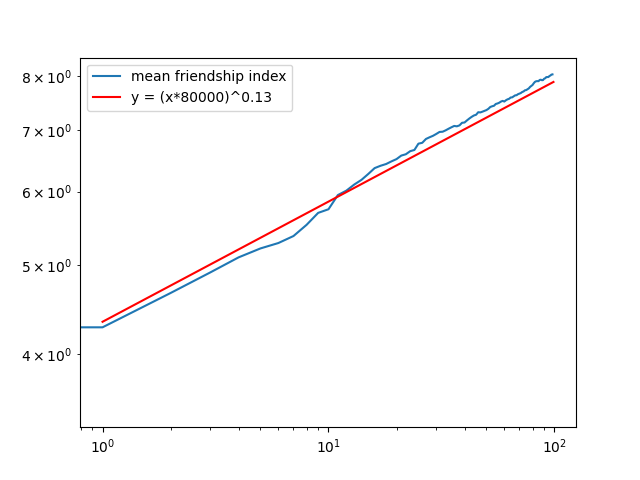
\includegraphics[scale=0.7]{diploma_results/dynamic_log/bap_mean_beta_4.png}
    \caption{Динамика среднего индекса дружбы  в\\ модели Барабаши"---Альберт\\ с пуассоновским распределением\\ степеней новых вершин \\ при $\lambda=4$}
\end{figure}
\begin{figure}[!ht]
    \centering
    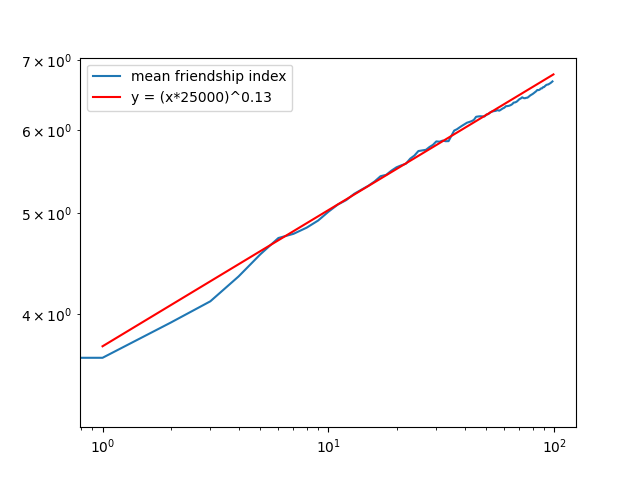
\includegraphics[scale=0.7]{diploma_results/dynamic_log/bap_mean_beta_5.png}
    \caption{Динамика среднего индекса дружбы  в\\ модели Барабаши"---Альберт\\ с пуассоновским распределением\\ степеней новых вершин \\ при $\lambda=5$}
\end{figure}
\begin{figure}[!ht]
    \centering
    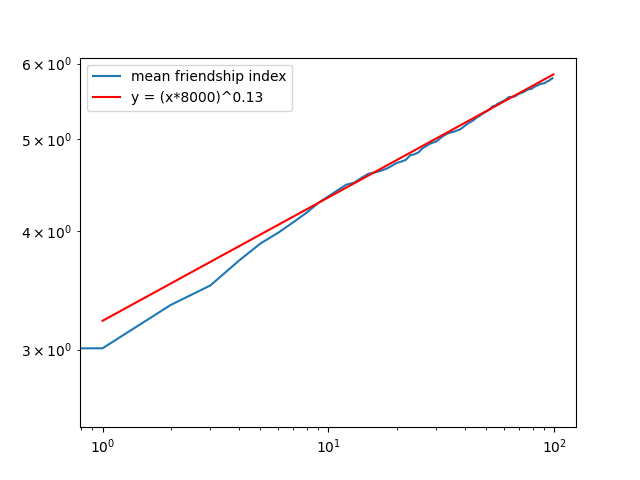
\includegraphics[scale=0.7]{diploma_results/dynamic_log/bap_mean_beta_6.png}
    \caption{Динамика среднего индекса дружбы  в\\ модели Барабаши"---Альберт\\ с пуассоновским распределением\\ степеней новых вершин \\ при $\lambda=6$}
\end{figure}
\begin{figure}[!ht]
    \centering
    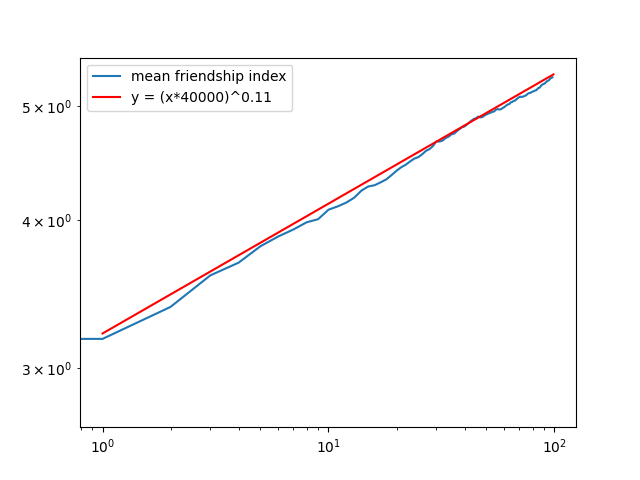
\includegraphics[scale=0.7]{diploma_results/dynamic_log/triad_mean_beta_3_0.25.png}
    \caption{Динамика среднего индекса дружбы  в\\ модели триадного замыкания\\ при $m=3$ и $p=0.25$}
\end{figure}
\begin{figure}[!ht]
    \centering
    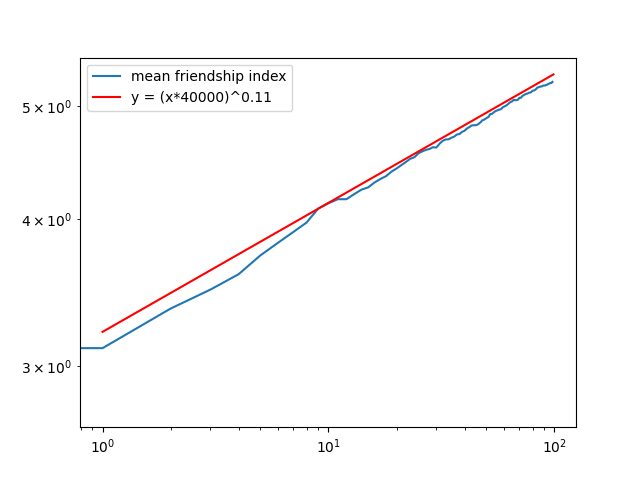
\includegraphics[scale=0.7]{diploma_results/dynamic_log/triad_mean_beta_3_0.5.png}
    \caption{Динамика среднего индекса дружбы  в\\ модели триадного замыкания\\ при $m=3$ и $p=0.5$}
\end{figure}
\begin{figure}[!ht]
    \centering
    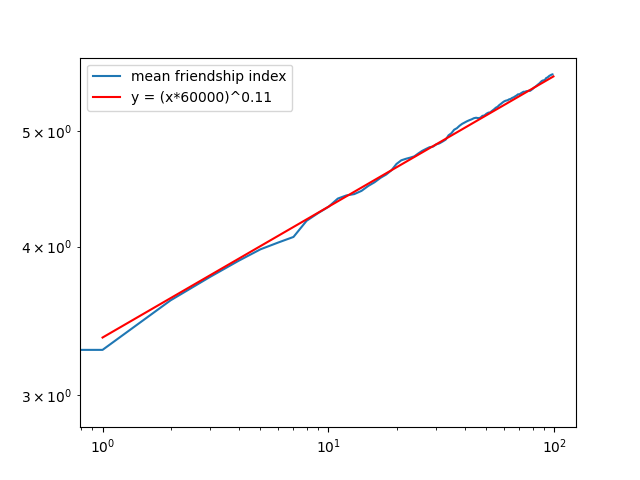
\includegraphics[scale=0.7]{diploma_results/dynamic_log/triad_mean_beta_3_0.75.png}
    \caption{Динамика среднего индекса дружбы  в\\ модели триадного замыкания\\ при $m=3$ и $p=0.75$}
\end{figure}
\begin{figure}[!ht]
    \centering
    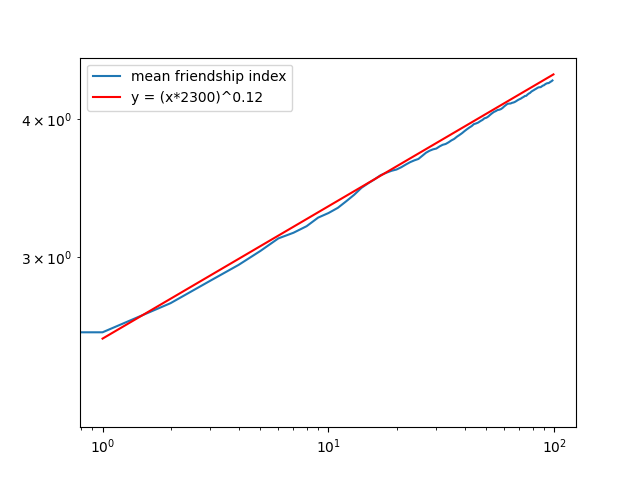
\includegraphics[scale=0.7]{diploma_results/dynamic_log/triad_mean_beta_5_0.25.png}
    \caption{Динамика среднего индекса дружбы  в\\ модели триадного замыкания\\ при $m=5$ и $p=0.25$}
\end{figure}
\begin{figure}[!ht]
    \centering
    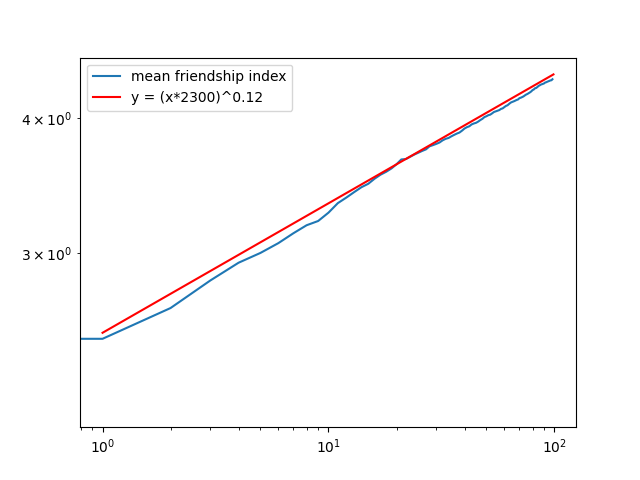
\includegraphics[scale=0.7]{diploma_results/dynamic_log/triad_mean_beta_5_0.5.png}
    \caption{Динамика среднего индекса дружбы  в\\ модели триадного замыкания\\ при $m=5$ и $p=0.5$}
\end{figure}
\begin{figure}[!ht]
    \centering
    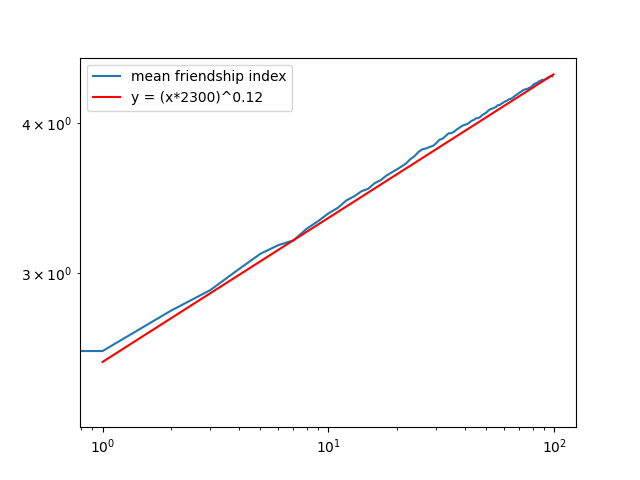
\includegraphics[scale=0.7]{diploma_results/dynamic_log/triad_mean_beta_5_0.75.png}
    \caption{Динамика среднего индекса дружбы  в\\ модели триадного замыкания\\ при $m=5$ и $p=0.75$}
\end{figure}
\section{Текст скрипта для отображения распределения индекса дружбы}\label{app:rgs}
\begin{minted}{python}
import igraph
import numpy as np
import matplotlib.pyplot as plt
import os
import multiprocessing 
import math
def static(name):
    file = open('\\source\\repos\\CSW\\real_graphs\\' + name + '.txt', 'r')
    res = []
    degrees = {}
    while True:
        line = file.readline()
        if not line:
            break
        edge = [int(j) for j in line.split(" ")]
        if not edge[0] in degrees:
            degrees[edge[0]] = 0
        degrees[edge[0]] += 1
        if not edge[1] in degrees:
            degrees[edge[1]] = 0
        degrees[edge[1]] += 1
    file.seek(0)
    sums = {}
    while True:
        line = file.readline()
        if not line:
            break
        edge = [int(j) for j in line.split(" ")]
        if not edge[0] in sums:
            sums[edge[0]] = 0
        sums[edge[0]] += degrees[edge[1]]
        if not edge[1] in sums:
            sums[edge[1]] = 0
        sums[edge[1]] += degrees[edge[0]]
    for i in degrees.keys():
        res.append(sums[i] / degrees[i] / degrees[i])
    file.close()
    bincnt = 100000
    ans = np.histogram(res, bincnt)
    x = ans[1]
    y = ans[0]
    x = np.resize(x, x.size - 1)
    plt.bar(x[0:int(bincnt / 100 * 2)], y[0:int(bincnt / 100 * 2)])
    plt.show()
    plt.clf()
if __name__ == "__main__":
    static('sx-askubuntu')
\end{minted}
\section{Текст скрипта для отображения динамики индекса дружбы}\label{app:rg}
\begin{minted}{python}
import igraph
import numpy as np
import matplotlib.pyplot as plt
import os
import multiprocessing 
import math
import datetime
def dynamics(name):
    file = open('\\source\\repos\\CSW\\real_graphs\\' + name, 'r')
    edge_list = []
    while True:
        line = file.readline()
        edge_list.append(line.split("\t"))
        if not line:
            break
    edge_list.pop()
    edge_list = [[i[0], 
                  i[1], 
                  datetime.datetime.strptime(i[3], '%Y-%m-%d %H:%M:%S').timestamp()] 
                 for i in edge_list]
    file.close()
    edge_list.sort(key = lambda i: i[2])
    step = 1000
    base = edge_list[0][2]
    res = []
    degrees = {}
    neibours_degrees = {}
    neibours = {}
    cnt = 0
    for i in edge_list:
        cnt += 1
        if not i[0] in degrees:
            degrees[i[0]] = 0
            neibours[i[0]] = set()
            neibours_degrees[i[0]] = 0
        if not i[1] in degrees:
            degrees[i[1]] = 0
            neibours[i[1]] = set()
            neibours_degrees[i[1]] = 0
        if i[0] == i[1]:
            degrees[i[0]] += 1
            neibours_degrees[i[0]] += degrees[i[0]]
            for j in neibours[i[0]]:
                neibours_degrees[j] += 1
            neibours[i[0]].add(i[0])
        else:
            degrees[i[0]] += 1
            degrees[i[1]] += 1
            if not i[1] in neibours[i[0]] and not i[0] in neibours[i[1]]:
                neibours_degrees[i[0]] += degrees[i[1]]
                neibours_degrees[i[1]] += degrees[i[0]]
            for j in neibours[i[0]]:
                neibours_degrees[j] += 1
            for j in neibours[i[1]]:
                neibours_degrees[j] += 1
            neibours[i[0]].add(i[1])
            neibours[i[1]].add(i[0])
        if (i[2] - base) >= step:
            base = step * math.ceil(i[2] / step)
            ans = []
            for j in degrees.keys():
                ans.append(neibours_degrees[j] / degrees[j] / degrees[j])
            res.append(np.mean(ans))
        # if cnt % step == 0:
        #     ans = []
        #     for j in degrees.keys():
        #         ans.append(neibours_degrees[j] / degrees[j] / degrees[j])
        #     res.append(np.mean(ans))
    plt.plot(res)
    plt.savefig("\\source\\repos\\CSW\\diploma_results\\" + name + "_iterational_dynamics.jpg")
    plt.clf()  
def run_thread(namegroup, i, res):
    ans = []
    for j in namegroup:
        ans.append(dynamics(j))
    res[i] = ans
def run(names):
    procs = []
    manager = multiprocessing.Manager()
    res = manager.dict()
    for (i, namegroup) in enumerate(names):
        p = multiprocessing.Process(target=run_thread, args=(namegroup, i, res))
        procs.append(p)
        p.start()
    for proc in procs:
        proc.join()
    ans = []
    for i in res.values():
        ans += i
    return ans
if __name__ == "__main__":
    # run([['askubuntu', 'askubuntu-a2q'], ['askubuntu-c2a', 'askubuntu-c2q'], ['mathoverflow', 'mathoverflow-a2q'], 
    #      ['mathoverflow-c2a', 'mathoverflow-c2q'], ['superuser', 'superuser-a2q'], ['superuser-c2a', 'superuser-c2q']])
    dynamics('soc-redditHyperlinks-body.tsv')
\end{minted}
\section{Текст скрипта для отображения динамики индекса дружбы в графах представленных в нескольких файлах}\label{app:rgp}
\begin{minted}{python}
import igraph
import numpy as np
import matplotlib.pyplot as plt
import os
import multiprocessing 
import math
import datetime
def dynamics(name):
    file = open('\\source\\repos\\CSW\\real_graphs\\' + name + '.txt', 'r')
    time_file = open('\\source\\repos\\CSW\\real_graphs\\' + name + '-dates.txt', 'r')
    times = {}
    while True:
        line = time_file.readline()
        if not line:
            break
        line = line.split("\t")
        line = [int(line[0]), int(line[1].replace('-', ''))]
        times[line[0]] = line[1]
    edge_list = []
    while True:
        line = file.readline()
        edge_list.append(line.split("\t"))
        if not line:
            break
    edge_list.pop()
    edge_list = [[int(j) for j in i] for i in edge_list]
    file.close()
    time_file.close()
    edge_list.sort(key = lambda i: times[i[0]] if i[0] in times else 100000000)
    step = 1000
    # base = edge_list[0][2]
    res = []
    degrees = {}
    neibours_degrees = {}
    neibours = {}
    cnt = 0
    for i in edge_list:
        cnt += 1
        if not i[0] in degrees:
            degrees[i[0]] = 0
            neibours[i[0]] = set()
            neibours_degrees[i[0]] = 0
        if not i[1] in degrees:
            degrees[i[1]] = 0
            neibours[i[1]] = set()
            neibours_degrees[i[1]] = 0
        if i[0] == i[1]:
            degrees[i[0]] += 1
            neibours_degrees[i[0]] += degrees[i[0]]
            for j in neibours[i[0]]:
                neibours_degrees[j] += 1
            neibours[i[0]].add(i[0])
        else:
            degrees[i[0]] += 1
            degrees[i[1]] += 1
            if not i[1] in neibours[i[0]] and not i[0] in neibours[i[1]]:
                neibours_degrees[i[0]] += degrees[i[1]]
                neibours_degrees[i[1]] += degrees[i[0]]
            for j in neibours[i[0]]:
                neibours_degrees[j] += 1
            for j in neibours[i[1]]:
                neibours_degrees[j] += 1
            neibours[i[0]].add(i[1])
            neibours[i[1]].add(i[0])
        # if (i[2] - base) >= step:
        #     base = step * math.ceil(i[2] / step)
        #     ans = []
        #     for j in degrees.keys():
        #         ans.append(neibours_degrees[j] / degrees[j] / degrees[j])
        #     res.append(np.mean(ans))
        if cnt % step == 0:
            ans = []
            for j in degrees.keys():
                ans.append(neibours_degrees[j] / degrees[j] / degrees[j])
            res.append(np.mean(ans))
    plt.plot(res)
    plt.savefig("\\source\\repos\\CSW\\diploma_results\\" + name + "_iterational_dynamics.jpg")
    plt.clf()
if __name__ == "__main__":
    # run([['askubuntu', 'askubuntu-a2q'], ['askubuntu-c2a', 'askubuntu-c2q'], ['mathoverflow', 'mathoverflow-a2q'], 
    #      ['mathoverflow-c2a', 'mathoverflow-c2q'], ['superuser', 'superuser-a2q'], ['superuser-c2a', 'superuser-c2q']])
    dynamics('cit-Patents')
\end{minted}

\section{Графики распределения и динамики индекса дружбы в реальных сетях}\label{app:real}
\begin{figure}[!ht]
    \centering
    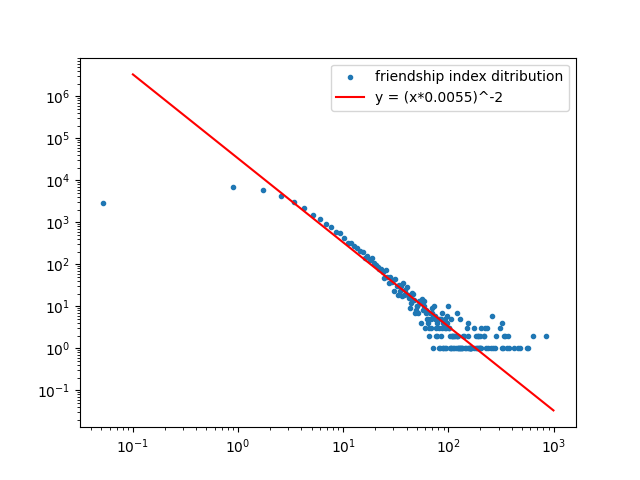
\includegraphics[scale=0.5]{diploma_results/static_real_log/Cit-HepPh.png}
    \caption{Распределение индекса дружбы  в\\ сети цитирования статей в сфере \\феноменологии физики высоких энергий\\ в логарифмической шкале}
\end{figure}
\begin{figure}[!ht]
    \centering
    \includegraphics[scale=0.5]{diploma_results/dynamic_real_log/Cit-HepPh_mean.png}
    \caption{Динамика индекса дружбы  в\\ сети цитирования статей в сфере \\феноменологии физики высоких энергий\\ в логарифмической шкале}
\end{figure}
\begin{figure}[!ht]
    \centering
    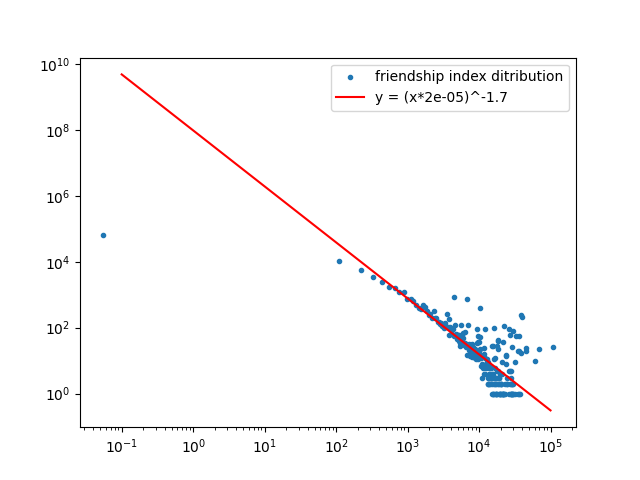
\includegraphics[scale=0.5]{diploma_results/static_real_log/gplus_combined.png}
    \caption{Распределение индекса дружбы  в\\ социальной сети Google+\\ в логарифмической шкале}
\end{figure}
\begin{figure}[!ht]
    \centering
    \includegraphics[scale=0.5]{diploma_results/dynamic_real_log/CollegeMsg_mean.png}
    \caption{Динамика индекса дружбы  в\\ сети сообщений студентов Калифорнийского университета в Ирвайне\\ в логарифмической шкале}
\end{figure}
\begin{figure}[!ht]
    \centering
    \includegraphics[scale=0.5]{diploma_results/static_real_log/CollegeMsg.png}
    \caption{Распределение индекса дружбы  в\\ сети сообщений студентов Калифорнийского университета в Ирвайне\\ в логарифмической шкале}
\end{figure}

\end{document}
